% 杭州电子科技大学本科毕业设计（论文）LaTeX模板
% 依据学校官方模板格式制作
\documentclass[a4paper,12pt,oneside,openany]{ctexbook}

% ==================== 页面设置 ====================
\usepackage{geometry}
\geometry{
    top=3cm,                % 对应【页边距】→ 上(T)：3厘米
    bottom=2cm,             % 对应【页边距】→ 下(B)：2厘米
    left=3cm,               % 对应【页边距】→ 左(L)：3厘米
    right=2cm,              % 对应【页边距】→ 右(R)：2厘米
    bindingoffset=1cm,      % 对应【页边距】→ 装订线(G)：1厘米，位置靠左
    % 页眉页脚布局（匹配Word【布局】选项卡）
    includehead,            % 页眉包含在上边距内（和Word原生逻辑完全一致）
    includefoot,            % 页脚包含在下边距内（和Word原生逻辑完全一致）
    headheight=15pt,        % 页眉内容固定高度（适配小五号字页眉，足够日常使用）
    headsep=0.5cm,          % 页眉底部→正文顶部的间距（匹配Word页眉距边界2cm）
    footskip=0.5cm,         % 正文底部→页脚顶部的间距（匹配Word页脚距边界1cm）
}

% ==================== 基础宏包 ====================
\usepackage{graphicx}
\usepackage{xcolor}
\usepackage{amsmath}
\usepackage{amssymb}
\usepackage{booktabs}
\usepackage{longtable}
\usepackage{array}
\usepackage{multirow}
\usepackage{float}
\usepackage[section]{placeins}
\usepackage{caption}
\usepackage{subcaption}
\usepackage{enumitem}
\usepackage{listings}
\usepackage{setspace}
\usepackage{fancyhdr}
\usepackage{titlesec}
\usepackage{tocloft}
\usepackage{indentfirst}
\usepackage{tabularx}
\usepackage{makecell}
\usepackage{ulem}
\usepackage{xeCJKfntef}

% ==================== 字体设置 ====================
% ctex已自动处理中文字体，此处设置英文字体
\setmainfont{Times New Roman}
\setCJKmainfont[AutoFakeBold=true]{SimSun} % 宋体，建议加上伪粗体
% 设置楷体
\setCJKfamilyfont{kai}[AutoFakeBold=true]{KaiTi} % 楷体

% ==================== 行距与段落 ====================
% 小四号字(12pt)，行距20磅（Word中行距20磅约等于1.39倍）
\setstretch{1.39}
\setlength{\parindent}{2em}

% ==================== hyperref（必须最后加载） ====================
\usepackage[
    colorlinks=true,
    linkcolor=black,
    citecolor=black,
    urlcolor=blue,
    bookmarks=true,
    bookmarksnumbered=true,
    unicode=true,
    pdftitle={基于用户画像与问答引导的“今天吃什么”智能推荐微信小程序设计},
    pdfauthor={作者姓名}
]{hyperref}

% ==================== 页眉页脚 ====================
\pagestyle{fancy}
\fancyhf{}
% 页眉：杭州电子科技大学本科毕业设计（论文），小五号宋体居中（9pt）
\fancyhead[C]{\zihao{-5} \songti 杭州电子科技大学本科毕业设计（论文）}
% 页脚：- 页码 -，五号Times居中
\fancyfoot[C]{\zihao{5} \normalfont -\thinspace\thepage\thinspace-}
\renewcommand{\headrulewidth}{0.4pt}
\renewcommand{\footrulewidth}{0pt}

% 章节起始页也使用fancy样式
\fancypagestyle{plain}{
\fancyhf{}
\fancyhead[C]{\zihao{-5} \songti 杭州电子科技大学本科毕业设计（论文）}
\fancyfoot[C]{\zihao{5} \normalfont -\thinspace\thepage\thinspace-}
\renewcommand{\headrulewidth}{0.4pt}
\renewcommand{\footrulewidth}{0pt}
}

% 页面样式：只有页眉，无页脚（用于目录）
\fancypagestyle{tocstyle}{
\fancyhf{}
\fancyhead[C]{\zihao{-5} \songti 杭州电子科技大学本科毕业设计（论文）}
\fancyfoot{}
\renewcommand{\headrulewidth}{0.4pt}
\renewcommand{\footrulewidth}{0pt}
}

% ==================== 标题格式设置 ====================
% 一级标题：黑体三号居中，段前0.5行（从页眉下方开始），段后2行
\ctexset{
chapter = {
format = \zihao{3}\heiti\centering,
beforeskip = 0.5\baselineskip,
afterskip = 2\baselineskip,
pagestyle = plain,
}
}

% 二级标题：黑体四号，靠左顶格，段前段后减少留白
\titleformat{\section}
{\zihao{4}\heiti}
{\thesection}
{1em}
{}
\titlespacing*{\section}{0pt}{0.5\baselineskip}{0.3\baselineskip}

% 三级标题：黑体小四号，靠左顶格，段前段后减少留白
\titleformat{\subsection}
{\zihao{-4}\heiti}
{\thesubsection}
{1em}
{}
\titlespacing*{\subsection}{0pt}{0.3\baselineskip}{0.2\baselineskip}

% ==================== 目录格式 ====================
\renewcommand{\cftchapfont}{\zihao{-4}\songti}
\renewcommand{\cftsecfont}{\zihao{-4}\songti}
\renewcommand{\cftsubsecfont}{\zihao{-4}\songti}
\renewcommand{\cftchapleader}{\cftdotfill{\cftdotsep}}
\renewcommand{\cftsecleader}{\cftdotfill{\cftdotsep}}
\renewcommand{\cftchappagefont}{\zihao{-4}}
\renewcommand{\cftsecpagefont}{\zihao{-4}}
\renewcommand{\cftsubsecpagefont}{\zihao{-4}}
\setlength{\cftbeforechapskip}{0.1\baselineskip}
\setlength{\cftbeforesecskip}{0pt}
\setlength{\cftbeforesubsecskip}{0pt}

% ==================== 图表标题格式 ====================
\captionsetup{
    font={small},
    labelfont={small},
    textfont={small},
    labelsep=quad,
    skip=0.5\baselineskip
}
\captionsetup[figure]{name={图}}
\captionsetup[table]{name={表}}

% ==================== 代码列表格式 ====================
\definecolor{codebg}{RGB}{248,248,248}
\definecolor{codeframe}{RGB}{200,200,200}
\definecolor{codecomment}{RGB}{0,128,0}
\definecolor{codestring}{RGB}{163,21,21}
\definecolor{codekeyword}{RGB}{0,0,255}

\lstset{
    language=Python,
    basicstyle=\zihao{5}\ttfamily,
    keywordstyle=\color{codekeyword}\bfseries,
    stringstyle=\color{codestring},
    commentstyle=\color{codecomment}\itshape,
    backgroundcolor=\color{codebg},
    frame=single,
    rulecolor=\color{codeframe},
    breaklines=true,
    showstringspaces=false,
    tabsize=4,
    numbers=left,
    numberstyle=\tiny\color{gray},
    numbersep=8pt,
    xleftmargin=2em,
    framexleftmargin=1.5em,
    aboveskip=1\baselineskip,
    belowskip=1\baselineskip,
    captionpos=b
}

% ==================== 参考文献格式 ====================
\makeatletter
\renewcommand{\@biblabel}[1]{[#1]\hfill}
\makeatother

% 定义上标引用命令
\newcommand{\super}[1]{\textsuperscript{#1}}

% ==================== 封面环境 ====================
\newenvironment{coverpage}{
    \clearpage
    \thispagestyle{empty}
    \zihao{4}
}{\clearpage}

% ==================== 文档开始 ====================
\begin{document}

% 全局设置前置部分为empty样式（封面、诚信承诺无页眉页脚）
\pagestyle{empty}

% ========== 封面 ==========
\thispagestyle{empty}
\begin{center}
% 学校名称图片
\vspace*{1cm}
\centerline{
  \hspace{-1.3cm} % 这里的数值控制左移量，可按需微调
  
\includegraphics[width=9.83cm,height=1.4cm,keepaspectratio]{images/school_title.png}
}

\vspace{1cm}

% 本科毕业设计（论文）- 35pt（约小一号），宋体，加粗
{\fontsize{35pt}{36pt}\songti\textbf{本科毕业设计（论文）}}

\vspace{0.5cm}

% （2026届）- 小二或二号，宋体，加粗
{\zihao{2}\songti\textbf{（2026届）}}

\vspace{1cm}

% 封面信息表格 - 标签：宋体小三加粗，内容：楷体小三不加粗
\renewcommand{\arraystretch}{1.8}
\begin{tabular}{@{}>{\zihao{-3}\bfseries\songti}r >{\zihao{-3}\kaishu}l@{}}
题\qquad 目 &
\CJKunderline{%
\parbox[b]{9cm}{
\centering
基于用户画像与问答引导的“今天吃什\\
么”智能推荐微信小程序设计
}%
} \\[0.15cm]
学\qquad 院 & \CJKunderline{\makebox[9cm][c]{计算机学院}} \\[0.15cm]
专\qquad 业 & \CJKunderline{\makebox[9cm][c]{计算机科学与技术}} \\[0.15cm]
班\qquad 级 & \CJKunderline{\makebox[9cm][c]{22052320}} \\[0.15cm]
学\qquad 号 & \CJKunderline{\makebox[9cm][c]{22051009}} \\[0.15cm]
学生姓名 & \CJKunderline{\makebox[9cm][c]{蔡炜权}} \\[0.15cm]
指导教师 & \CJKunderline{\makebox[9cm][c]{潘玉剑}} \\[0.15cm]
完成日期 & \CJKunderline{\makebox[9cm][c]{2026年4月}} \\
\end{tabular}

\vfill
\end{center}
\clearpage

% ========== 诚信承诺书 ==========
\newpage
\thispagestyle{empty}
\begin{center}
\vspace*{3.5cm}

% 标题：小二号字，黑体，加粗，字间空两个全角空格
{\zihao{-2}\heiti\textbf{诚\quad 信\quad 承\quad 诺}}

\vspace{0.5cm}
\end{center}

% 正文：四号字，宋体，不加粗
\zihao{4}\songti
\setlength{\parindent}{2em}
我谨在此承诺：本人所写的毕业论文《\uline{\hspace{0.3em}基于用户画像与问答引导的“今天吃什么”智能推荐微信小程序设计\hspace{0.3em}}》均系本人独立完成，没有抄袭行为，凡涉及其他作者的观点和材料，均作了注释，若有不实，后果由本人承担。

\vspace{1cm}

% 签名部分：小三号字，黑体加粗标签，宋体日期
\begin{flushright}
\zihao{-3}\songti
\setlength{\parindent}{0em}
{\heiti\textbf{承诺人（签名）：}}\CJKunderline{\makebox[5cm]{}}

\vspace{1cm}

{\songti 2026年 5月 12日}
\end{flushright}
\clearpage

% ========== 中文摘要 ==========
\clearpage
\thispagestyle{tocstyle} % 使用带页眉的样式

\begin{center}
\vspace*{-0.5\baselineskip}
{\zihao{3}\heiti 摘\quad 要}
\end{center}
% 摘要不加入目录
\zihao{-4}\songti

高校及周边的餐饮选择看似丰富，实际上候选太多反而让人犹豫不决，尤其是时间紧、预算有限或者身体状态特殊的时候。本文设计了一款微信小程序，通过几个简单问题了解用户当下的用餐场景（时段、预算、人数、口味、身体状态等），再结合用户填写的长期画像（健康目标、饮食禁忌、口味偏好等），给出可执行的菜品推荐。

推荐过程先按预算、审核状态和忌口过滤掉不可行的选项，再用 sentence-transformers 模型计算用户和菜品的语义相似度，最后综合距离、历史重复度和特殊状态等因素排序。系统前端是微信小程序，后端基于 FastAPI 和 MySQL 构建，支持完整的注册登录、画像编辑、问答交互、推荐展示、选择确认和历史回看流程。测试表明，系统能在较短时间内返回符合当前场景的推荐结果，预算控制、饮食禁忌过滤和地理位置约束都执行得比较到位。

\vspace{\baselineskip}
\noindent\textbf{\heiti\zihao{-4}关键词：}{\zihao{-4}\songti 智能推荐；用户画像；问答引导；微信小程序；餐饮推荐}

% ========== 英文摘要 ==========
\clearpage
\thispagestyle{tocstyle} % 使用带页眉的样式
\begin{center}
\vspace*{-0.5\baselineskip}
{\zihao{3}\bfseries ABSTRACT}
\end{center}
% ABSTRACT不加入目录
\zihao{-4}\normalfont

In campus and surrounding areas, choosing what to eat appears easy due to abundant options, yet the large candidate pool often leads to decision paralysis, especially when users are short on time, have a tight budget, or face special physical conditions. This thesis presents a WeChat Mini Program that asks a few lightweight questions about the current dining context (meal time, budget, number of diners, taste preference, physical state) and combines them with the user's long-term profile (health goals, dietary restrictions, taste preferences) to generate actionable dish recommendations.

The recommendation pipeline consists of three stages: hard filtering first removes dishes that violate budget, approval status, or dietary taboos; semantic recall then computes cosine similarity between user and dish vectors generated by a local sentence-transformers model; finally, a re-ranking stage fuses semantic similarity, distance penalty, and history smoothing to balance relevance, accessibility, and diversity. The backend is built with FastAPI and MySQL, while the frontend is a WeChat Mini Program supporting registration, profile editing, questionnaire-based recommendation, result confirmation, and history review. Experimental results show that the system returns context-consistent recommendations within acceptable latency, with budget compliance, dietary constraints, and geographical accessibility all performing well.

\vspace{\baselineskip}
\noindent\textbf{\zihao{-4} Keywords: }{\zihao{-4} recommender system; user profile; questionnaire guidance; WeChat Mini Program; food recommendation}

% ========== 目录 ==========
\clearpage
\thispagestyle{tocstyle} % 使用目录专用样式（有页眉无页脚）
\begin{center}
\vspace*{-0.5\baselineskip}
{\zihao{3}\heiti 目\quad 录}
\vspace*{-4\baselineskip}
\end{center}

% 取消\tableofcontents自动生成的标题
\renewcommand{\contentsname}{} 
\zihao{-4}
\tableofcontents
\clearpage

% ========== 正文：页眉+页码 ==========
\pagestyle{fancy}
\pagenumbering{arabic}
\setcounter{page}{1}

% ========== 正文各章 ==========
% 第一章 绪言
\chapter{绪言}

\section{研究背景}

随着移动互联网、本地生活服务平台与即时配送体系的成熟，用户在餐饮选择上拥有了前所未有的丰富供给。以美团、饿了么、大众点评为代表的本地生活平台聚合了数以万计的餐饮商户，用户在手机端即可浏览海量菜品信息。对于高校场景而言，食堂、校内商户、校外餐馆、外卖平台与便利食品共同构成了高密度、多样化的候选集合。表面上看，候选数量增加意味着用户有更大概率找到符合口味与价格预期的餐品；但从决策行为角度分析，候选扩张同时也显著提高了用户的选择成本，尤其在时间紧迫、预算有限或身体状态波动明显时，这种成本会进一步放大。

诺贝尔经济学奖得主赫伯特·西蒙（Herbert Simon）提出的"有限理性"理论指出，决策者在信息过载环境中难以对所有选项进行完全理性的评估，往往会采用启发式策略或陷入决策瘫痪\textsuperscript{[1]}。在餐饮选择场景中，这一现象表现得尤为明显：当用户面对数十甚至上百个候选菜品时，"选择困难"不仅消耗时间，还会带来心理负担。特别是在高校场景中，学生群体具有用餐时间集中、预算敏感、健康意识增强等特点，对推荐系统的即时性和可执行性提出了更高要求。

餐饮推荐与传统商品推荐存在明显差异。商品推荐（如电商平台的商品推荐）通常以长期偏好和历史行为为主要依据，用户购买决策周期较长，且对即时约束的要求相对较低。而餐饮推荐更强调即时决策与现实约束的协调：用户在同一天内可能因为时段、天气、情绪、身体状态或同伴关系而改变饮食偏好。例如，早餐倾向清淡，夜宵偏好高热量或重口味；减脂阶段更关注低油低糖，胃部不适时则倾向温和饮食；单人用餐追求便捷，聚餐场景则注重菜品的丰富性与分享性。因此，单纯依靠历史点击或购买记录进行推荐，往往会出现"偏好相近但场景不适"的问题，导致推荐结果在理论上合理、在现实中却难以执行。

在此背景下，构建一套能够显式捕捉当前场景、并对预算、禁忌与距离进行约束优化的餐饮推荐系统，具有较强的现实意义。本文所研究的问题并非泛化意义上的"美食推荐"，而是面向"当前想吃什么"这一即时决策任务，目标是在较短交互成本下输出可执行、可解释且场景一致的推荐结果。

\section{国内外研究现状}

\subsection{推荐系统基础方法研究}
经过多年发展，推荐系统已形成较为成熟的技术体系。在早期研究中，协同过滤与基于内容的推荐是两种最具代表性的方法。协同过滤依托用户与物品之间的交互行为挖掘相似关系，进而完成个性化推荐，其中又分为基于用户的协同过滤与基于物品的协同过滤两类典型实现方式\super{[2]}。不过，协同过滤方法高度依赖历史交互数据，在用户行为稀疏或新用户、新物品较多的场景下，推荐效果会出现明显下降。基于内容的推荐则以物品自身属性为依据，通过提取特征并匹配用户历史偏好完成推荐，可解释性较强，但也容易陷入推荐范围固化、结果同质化的问题，难以发掘用户的潜在兴趣\super{[3]}。

随着数据规模扩大与深度学习技术的普及，矩阵分解、神经协同过滤、注意力机制以及图神经网络等方法被广泛引入推荐领域，进一步提升了模型的特征表达与泛化能力。Koren等人提出的矩阵分解技术，通过对用户—物品交互矩阵进行低维分解，有效改善了数据稀疏带来的影响\super{[4]}。He等人提出的神经协同过滤模型，使用多层感知机替代传统线性内积，让模型能够更好地拟合用户与物品之间的非线性交互关系\super{[5]}。近几年，基于Transformer的序列推荐模型得到快速发展，例如SASRec、BERT4Rec等方法借助自注意力机制捕捉用户行为序列中的时序依赖，在公开数据集上展现出更优的推荐性能\super{[6]}。

\subsection{餐饮推荐与本地生活推荐研究}
在餐饮及本地生活服务场景中，推荐思路逐渐从静态偏好建模转向上下文感知推荐。与传统推荐场景不同，餐饮消费受时间、位置、环境、社交关系等实时因素影响明显，将这些情境信息融入模型，能够有效提升推荐结果的实用性。Adomavicius等人将上下文信息归纳为用户、物品与交互三大类别，并搭建了多维上下文感知的推荐框架\super{[7]}。

在地理位置相关研究中，用户与商家的空间距离是影响餐饮选择的重要因素。Liu等人在矩阵分解模型中加入地理影响因子，利用距离衰减规律刻画用户的实际活动范围\super{[8]}。Yin等人基于用户历史签到数据建模位置偏好，证实了餐饮选择中存在显著的空间聚集特征\super{[9]}。在文本特征利用方面，菜品名称、口味标签、食材构成与描述文本都可作为有效特征。Zhang等人采用Word2Vec对菜品文本进行向量表示，结合用户评论文本构建语义匹配模型，使召回结果更贴合用户偏好\super{[10]}。在健康导向推荐方面，部分研究将热量、营养成分等指标加入优化目标，为有特殊饮食需求的用户提供更具针对性的推荐服务\super{[11]}。

\subsection{交互式推荐与问答引导研究}
交互式推荐与对话式推荐是近年来的研究热点，其核心思路是通过主动交互补充用户偏好信息，而不是被动依赖历史行为。在用户信息不足时，系统可通过提问、对话等方式快速获取关键偏好，快速构建有效的推荐依据。Christakopoulou等人基于强化学习设计对话推荐策略，动态选择提问内容以最大化信息获取效率\super{[12]}。Zhang等人提出基于属性选择的交互推荐框架，通过多轮提问逐步缩小候选范围，提升推荐精准度\super{[13]}。

在餐饮推荐场景中，问答式交互具备天然优势。就餐相关的约束条件相对明确，包括预算、口味、距离、饮食禁忌等，用户通常可以快速完成结构化作答。相关研究表明，仅通过3—5个关键问题的轻量交互，就能明显缩小候选范围并提升用户体验\super{[14]}。但目前多数交互式餐饮推荐工作仍停留在算法验证阶段，对前后端系统联动、交互日志记录与工程落地等实际问题考虑不足，距离实际可用的系统仍有差距。

\subsection{现有研究的不足与本文定位}

综合上述研究现状，现有工作存在以下不足：

\begin{enumerate}[label=\arabic*., leftmargin=2em, itemsep=0.2em]
    \item \textbf{约束建模与偏好建模脱节}：多数系统侧重于提升推荐结果的偏好匹配度，而对预算、距离、禁忌等硬性约束的执行性关注不足，导致推荐结果"好看但不可用"。
    \item \textbf{长期偏好与即时场景割裂}：传统推荐系统过度依赖历史行为，难以适应用户在同一天内的偏好波动；而纯问答系统又忽略了用户的长期特征，导致推荐缺乏个性化基础。
    \item \textbf{工程闭环不完整}：很多研究停留在算法原型阶段，缺少完整的前端交互、后端服务、数据存储与日志回流机制，难以形成可持续迭代的产品。
\end{enumerate}

针对上述问题，本文提出了一种融合静态画像与即时问答的双通道建模方法，并采用"硬性过滤---向量召回---综合重排"的三阶段推荐策略，在保证约束可执行的前提下提升语义相关性。同时，本文完成了微信小程序前端、FastAPI 后端、MySQL 数据存储与向量化模块的完整工程实现，形成了从需求采集到结果反馈的闭环链路。

\section{本文的研究目标和内容}

为了让高校及周边用户在面对"今天吃什么"这一高频决策问题时能够快速获得符合当前场景的可执行推荐，本文设计并实现了一套基于用户画像与问答引导的智能推荐微信小程序。该系统包括面向用户的微信推荐小程序、基于 FastAPI 的后端服务与数据管理平台，以及融合语义向量与约束排序的智能推荐引擎。

本文主要研究内容包括以下几个方面：

\textbf{（1）设计并实现微信推荐小程序。}通过分析高校用户在餐饮选择中的核心痛点（候选过载、场景多变、约束复杂），确定小程序以"即时场景采集+可执行推荐"为核心定位；学习微信小程序开发技术，设计"首页---问答---推荐---确认---历史"的闭环交互流程，实现用户注册登录、即时问答引导、推荐结果展示、选择确认与历史回看等功能；结合微信定位 API，支持基于地理位置的附近美食浏览，为用户提供从决策到执行的完整链路。

\textbf{（2）设计并实现后端服务与数据管理平台。}基于 FastAPI 框架构建高性能的 RESTful API 服务，按业务职责划分为认证、画像、菜品、推荐与日志五大模块；使用 SQLAlchemy ORM 完成数据库建模，采用 MySQL 持久化存储用户、画像、菜品、店铺、历史记录和交互日志；设计基于 JWT 的鉴权机制保障接口安全，实现前后端分离的分层架构，使系统具备良好的可维护性与可扩展性。

\textbf{（3）研究基于用户画像与问答引导的推荐方法，分析传统推荐算法在即时餐饮场景中的不足。}在研究语义向量召回与约束排序的基础上，针对传统协同过滤和基于历史行为的推荐方法在"冷启动""场景失配"等方面的问题，提出"静态画像+即时问答"的双通道建模思路；设计"硬性过滤---向量召回---综合重排"的三段式推荐策略，将预算、禁忌、距离等硬性约束前置执行，再通过语义向量捕捉用户当前意图，最后融合距离惩罚与历史平滑进行综合排序，使推荐结果兼顾可执行性与场景一致性。

\textbf{（4）设计并实现菜品向量化与语义召回模块。}在采集菜品的多维属性信息（菜名、菜系、口味标签、食材、描述等）后，基于 sentence-transformers 本地模型将结构化字段拼接为语义文本并编码为稠密向量；融合用户静态画像（长期偏好、健康目标、饮食禁忌）与即时问答（用餐时段、预算、口味强度、特殊状态）构建用户目标向量，通过余弦相似度计算实现语义召回；引入特殊状态加权机制（如减脂、胃不舒服等场景），对召回结果进行场景化增强，提升推荐结果与当前状态的匹配度。

\textbf{（5）设计并实现数据闭环与测试验证机制。}建立交互日志体系，记录推荐曝光、点击、确认和负样本行为，形成"采集---推荐---反馈---回流"的数据闭环；开展功能测试验证各模块正确性，开展场景化测试验证推荐算法在不同预算、时段、特殊状态下的适配能力，开展性能测试与鲁棒性测试验证系统的响应速度与异常处理能力，确保系统具备工程可用性。

\section{论文组织结构}

全文共五章，各章内容安排如下：

\textbf{第一章 绪言}。介绍研究背景、国内外研究现状、研究意义与目的、研究内容与技术路线，以及论文组织结构。

\textbf{第二章 系统相关技术概述}。介绍推荐系统基本原理、微信小程序开发技术、FastAPI 后端框架、SQLAlchemy ORM 技术、MySQL 数据库、sentence-transformers 向量化技术以及 JWT 鉴权机制，并对关键技术选型进行对比分析。

\textbf{第三章 系统设计与实现}。阐述系统需求分析、总体架构设计、数据库设计、核心模块详细设计（认证、画像、菜品、推荐、历史日志）、前端交互实现，并给出关键流程图与界面说明。

\textbf{第四章 系统功能测试}。给出测试目标与测试环境、系统功能性测试、场景化推荐测试、非功能性测试（性能、可靠性、易用性、鲁棒性）以及测试结论。

\textbf{第五章 总结与展望}。总结全文工作，分析主要特点与创新点，指出存在的问题，并提出后续改进方向。

% 第二章 系统相关技术概述
\chapter{系统相关技术概述}

本章对"今天吃什么"智能推荐系统所依赖的理论基础与关键技术进行系统阐述。首先介绍推荐系统的基本范式与餐饮推荐的特殊约束，继而分析主流推荐算法的原理与局限；随后分别从前端、后端、数据库、文本向量化及安全认证五个维度，深入剖析各技术的核心机制，并结合本项目的业务特征论证技术选型的合理性，为后续系统设计与实现奠定理论基础。

\section{推荐系统基本原理}

\subsection{推荐系统的定义与目标}

推荐系统（Recommender System）本质上是一种信息过滤机制，其核心任务是在用户集合 $U$ 与物品集合 $I$ 构成的二元空间上，学习一个评分映射函数 $f: U \times I \rightarrow \mathbb{R}$，使得对于特定用户 $u \in U$，系统能够从其尚未交互过的物品子集 $I_u^- = I \setminus I_u^+$ 中筛选出预测评分最高的前 $N$ 个物品，形成个性化推荐列表 $R_u$。形式化表达为：

\begin{equation}
R_u = \mathop{\arg\max}_{i \in I_u^-} f(u, i)
\end{equation}

该定义揭示了推荐系统的两个核心目标：一是准确性，即推荐结果应尽可能贴合用户的真实偏好；二是覆盖率，即系统应能够在海量候选中有效挖掘长尾物品，避免推荐结果过度集中于热门项目。在餐饮推荐场景中，这一目标还需进一步受限于预算、距离、饮食禁忌等现实条件，使得评分函数 $f$ 不再仅仅是偏好强度的度量，而是可执行性的综合评估。项亮在《推荐系统实践》中系统阐述了推荐系统的工程化方法，涵盖从数据采集、特征工程到算法评估的完整流程\super{[16]}。

\subsection{推荐系统的典型架构}
在实际应用中，工业级推荐系统大多采用多阶段级联的架构形式，以此平衡计算效率与推荐精准度。整体架构通常分为召回、粗排、精排和重排四个环节。召回阶段的主要任务是快速筛选候选，从海量物品库中提取出上千条相关候选，常用方式包括协同过滤召回、向量相似度召回和规则标签召回等，这一阶段更注重筛选速度与覆盖范围，允许存在少量精度损失。粗排阶段会对召回结果做初步精简，借助逻辑回归、浅层神经网络等轻量模型快速打分，把候选规模压缩到合适范围，减少后续精排的计算压力。精排是提升推荐效果的关键环节，通过DeepFM、DIN等复杂深度学习模型，对候选菜品进行精细化个性化打分，充分挖掘用户与物品之间的关联特征。最后的重排阶段，会结合业务规则对结果做优化调整，例如控制推荐多样性、平衡菜品新鲜度、避免重复推荐，同时加入硬性约束过滤，最终生成可直接展示给用户的推荐列表。

这种多阶段分层架构的核心思路，是把不同复杂度的计算任务分配到对应阶段，在保证响应速度的前提下提升推荐效果。本系统所采用的“硬性过滤—向量召回—综合重排”策略，正是对该架构的轻量化适配，先通过规则约束保证推荐可用，再利用语义向量提升匹配精度，最后结合多目标因素完成排序优化。

\subsection{餐饮推荐的特殊性}
与电商、新闻等常见推荐场景相比，餐饮推荐具备鲜明的领域特点，这些特点也直接决定了系统的设计方向。首先，餐饮推荐具有较强的约束性，用户的就餐选择会被预算、距离、营业状态、饮食禁忌等条件严格限制，任何超出约束范围的推荐都不具备实际使用价值。其次，餐饮需求具有明显的时效性，用户在早午晚餐、夜宵等不同时段的偏好差异较大，即使是同一时段，也会因身体状态、心情变化产生不同需求，单纯依靠历史行为很难适配这种动态变化。再次，餐饮消费的容错率较低，一旦完成点餐，后续修改或更换的成本较高，因此对推荐结果的准确性要求更高。最后，餐饮推荐需要兼顾多目标平衡，用户通常会同时考虑口味、健康、价格、距离等多个因素，系统需要在这些维度之间做好权衡，而不是只优化单一指标。

结合这些特点，本系统没有采用仅依赖历史行为的协同过滤方案，而是采用静态画像结合即时问答的双通道建模方式，通过主动交互获取当前场景信息，并将硬性约束放在推荐流程的前端，保证最终结果符合实际使用场景。

\section{常用推荐算法分析}
\subsection{基于内容的推荐算法}
基于内容的推荐算法，核心是依靠物品自身的属性特征与用户的历史偏好做匹配。具体实现时，系统会先提取物品的关键特征，构建物品特征向量；同时根据用户的点击、收藏、下单等历史行为，总结出用户的兴趣偏好向量；最后通过计算两种向量的相似度，把相似度较高的物品推荐给用户。在餐饮场景中，菜品的菜系、口味、食材、价格、营养成分等，都可以作为特征参与计算。

这种算法的优势在于，用户建模相互独立，不会受其他用户数据的干扰，新上架的菜品也能立刻参与推荐，不存在物品冷启动的问题。但它也存在明显局限，推荐结果会被用户的历史偏好限制，很难挖掘用户潜在的兴趣点，容易出现推荐内容同质化的问题；同时对于没有任何行为记录的新用户，无法构建偏好模型，仍然会遇到用户冷启动的难题。在本系统中，基于内容推荐的思想主要应用在菜品向量化部分，通过提取菜品的多维属性生成语义向量，为后续的相似度计算提供支撑。周志华在《机器学习》中系统介绍了各类学习算法的原理与适用场景，为本系统的算法选型提供了理论参考\super{[17]}。


\subsection{协同过滤推荐算法}

协同过滤（Collaborative Filtering, CF）是当前应用最为广泛的推荐算法之一，其核心假设是"兴趣相似的用户倾向于偏好相似的物品"。该算法不依赖物品本身的内容特征，而是基于用户与物品之间的交互矩阵（如评分矩阵或隐式反馈矩阵）进行建模。从实现路径上，协同过滤可分为基于用户的协同过滤（User-based CF）与基于物品的协同过滤（Item-based CF）两类。

基于用户的协同过滤首先计算目标用户与其他用户之间的相似度（常用皮尔逊相关系数或余弦相似度），选取相似度最高的 $K$ 个用户作为近邻集合；随后根据近邻用户对候选物品的评分预测目标用户的偏好程度，将预测评分最高的物品予以推荐。基于物品的协同过滤则转换视角，先计算物品之间的共现相似度（即同时被同一用户偏好的概率），再根据目标用户历史喜欢的物品，推荐与其历史物品相似度最高的其他物品。

协同过滤算法能够突破用户既有兴趣边界的限制，通过群体行为发现潜在关联，对长尾物品的挖掘能力较强。但其固有缺陷在于：新用户或新物品因缺乏历史交互数据而难以被有效建模，即冷启动问题；随着用户规模和物品 catalog 的增长，用户-物品交互矩阵会极度稀疏，导致相似度计算失真；此外，算法对数据规模高度敏感，初期数据不足时推荐质量难以保证。考虑到本系统面向的是即时决策场景，用户的历史餐饮记录有限且场景波动大，单纯依赖协同过滤难以适应"当前想吃什么"这一动态需求，因此本系统将其作为辅助思路，而非核心推荐策略。李航在《统计学习方法》中对监督学习的主要模型做了严密的数学推导与算法总结，其中的分类与回归方法为本系统的评分预测提供了方法论基础\super{[18]}。

\subsection{混合推荐策略}

混合推荐并非一种独立的算法，而是将多种推荐算法按照特定策略进行组合，以发挥各自优势、弥补单一算法的不足。常见的组合模式包括加权融合、层叠过滤、特征扩充与元级联等。加权融合模式并行执行多种算法，通过线性加权整合各算法的预测得分；层叠模式则采用串行结构，先以一种算法生成候选集合，再以另一种算法对候选进行精细化筛选或重排；特征扩充模式将一种算法生成的中间特征作为另一种算法的输入，实现信息互补。

本系统采用的推荐策略属于层叠混合模式，具体表现为"硬性过滤---向量召回---综合重排"的三段式流水线。第一阶段基于规则进行硬性过滤，利用预算区间、审核状态及饮食禁忌等约束条件快速剔除不可执行候选，缩小搜索空间；第二阶段基于语义向量进行相似度召回，捕捉用户当前意图与菜品属性之间的语义关联；第三阶段综合语义相似度、距离衰减与历史平滑等因素进行重排序，实现多目标权衡。这种分层架构既保证了约束的严格满足，又通过向量语义提升了推荐的精准度，同时避免了单一算法在复杂场景下的局限性。

\section{前端开发技术}

\subsection{微信小程序技术架构}
微信小程序是腾讯在2017年推出的轻量级应用形式\super{[19]}，它采用逻辑层与渲染层相互分离的双线程架构。其中，逻辑层基于独立的JavaScript引擎JSCore运行，主要负责处理业务逻辑、管理数据状态以及发起网络请求；渲染层则负责页面的视觉渲染，使用WXML描述页面结构，通过WXSS定义页面样式。两层之间无法直接通信，而是借助底层Native提供的JSBridge机制完成异步数据交互，逻辑层通过`setData`方法将数据更新传递到渲染层，从而触发页面重新渲染。

这种双线程隔离的设计带来了两方面突出优势。一方面提升了运行安全性，由于逻辑层不具备完整的DOM操作权限，开发者无法直接操作页面节点，能够有效避免XSS注入等前端安全风险。另一方面优化了渲染性能，WXML和WXSS代码经过编译后由Native层直接解析渲染，减少了传统WebView中频繁的DOM计算与页面重绘，提升了页面流畅度。同时，微信小程序提供了网络请求、本地存储、地理位置、扫码等丰富的原生接口，开发者可以通过统一的API快速调用系统能力，降低功能实现难度。

在组件开发方面，小程序内置了视图容器、基础控件、表单、导航等常用组件，同时支持自定义组件的封装与复用。在样式适配方面，WXSS使用rpx作为自适应单位，以屏幕宽度750rpx为基准进行等比缩放，能够自动适配不同分辨率的移动设备，有效降低了多机型适配的开发成本。

\subsection{微信小程序在本项目中的适用性分析}
本系统最终选用微信小程序作为前端展示载体，主要结合了目标用户场景与实际开发效率两方面因素。从用户使用角度来看，高校学生几乎都在使用微信，小程序无需下载安装、即用即走的特点，大幅降低了用户的使用门槛；同时小程序支持消息订阅和社交分享，便于在用餐高峰时段向用户推送推荐内容，提升系统使用率。从技术实现角度来看，小程序的双线程架构可以稳定支撑问答交互页面的分步操作和推荐结果页面的动态加载，其原生提供的地理位置接口能够直接获取用户经纬度，为后续距离计算和附近美食推荐提供了可靠的数据来源。此外，微信小程序拥有完善的开发者工具，支持代码编写、真机调试和性能监控，能够满足本项目从开发、调试到测试的完整工程需求。


\section{后端开发框架}

\subsection{FastAPI 框架技术原理}

FastAPI 是基于 Python 3.7 及以上版本类型注解构建的现代 Web 框架\super{[20]}，其底层建立在 Starlette ASGI 工具包与 Pydantic 数据验证库之上。ASGI（Asynchronous Server Gateway Interface）是 Python 异步服务器网关接口标准，相较于传统的 WSGI（Web Server Gateway Interface），ASGI 原生支持异步非阻塞 I/O 操作，使得框架能够在单线程内通过事件循环（Event Loop）并发处理大量连接，显著提升了 I/O 密集型场景下的吞吐量。

FastAPI 的核心设计哲学是将 Python 的类型系统（Type Hints）作为一等公民。开发者在路由处理函数的参数中声明数据类型后，FastAPI 自动利用 Pydantic 完成请求体的解析、校验与序列化。Pydantic 通过 Python 的类型注解在运行时构建数据模型，对传入的 JSON 数据进行严格的类型检查与约束验证，一旦数据不符合模型定义，框架会自动返回结构化的 422 错误响应，无需开发者编写冗余的校验代码。这种类型驱动开发模式不仅减少了样板代码，还使得接口的数据契约具有自文档化特性。

在依赖管理方面，FastAPI 提供了基于 \texttt{Depends} 装饰器的依赖注入系统。开发者可以将数据库会话获取、用户身份校验、权限检查等横切关注点封装为依赖函数，通过声明式的方式注入到路由处理函数中。这种设计实现了业务逻辑与基础设施的解耦，使得代码具有更好的可测试性与可复用性。此外，FastAPI 内置对 OpenAPI 与 JSON Schema 的自动生成支持，服务启动后会自动暴露交互式 API 文档（Swagger UI 与 ReDoc），前端开发者可直接在浏览器中查看接口定义、参数结构并发起调试请求，显著提升了前后端协作效率。

\subsection{SQLAlchemy ORM 技术}

SQLAlchemy 是 Python 生态中功能较为完备的对象关系映射（ORM）工具集，其设计理念是在保持关系型数据库完整表达能力的同时，提供高层次的数据操作接口。SQLAlchemy 的 ORM 层采用声明式映射（Declarative Mapping）模式，允许开发者通过定义 Python 类来描述数据库表结构，类的属性对应表的列，类实例对应表中的行记录，从而将数据库操作转化为直观的面向对象操作。

在会话管理方面，SQLAlchemy 通过 Session 对象实现单元工作模式（Unit of Work）。Session 作为对象与数据库之间的持久化上下文，跟踪所有待持久化对象的状态变更，并在事务提交时（\texttt{session.commit()}）将变更批量同步至数据库；若操作过程中发生异常，可通过回滚（\texttt{session.rollback()}）撤销未提交的变更，确保数据一致性。此外，SQLAlchemy 内置连接池（Connection Pool）机制，对数据库连接进行复用与管理，避免了频繁创建连接带来的性能开销。

SQLAlchemy 的另一重要特性是数据库无关性。通过更换连接字符串与方言（Dialect）配置，同一套 ORM 代码可无缝迁移至 MySQL、PostgreSQL、SQLite 等不同数据库后端，这种抽象能力为开发环境与生产环境的灵活部署提供了便利。在本系统中，SQLAlchemy 的声明式基类被用于定义用户、画像、菜品、店铺、历史记录等核心实体模型，并通过外键关系与级联操作实现了实体间的关联建模。

\subsection{后端技术选型分析}

在 Python Web 开发领域，FastAPI、Flask 与 Django 是三种主流框架，三者在设计理念与适用场景上存在显著差异。Flask 作为微框架，核心功能精简，扩展依赖第三方库，学习曲线平缓，适合快速原型开发，但缺乏原生异步支持与自动文档生成能力，大型项目中需自行整合校验、路由及文档工具。Django 作为全栈框架，内置 ORM、管理后台、认证系统等完整功能，适合内容密集型的大型应用，但其同步架构与较重的框架包袱对于轻量级 API 服务而言显得冗余，且学习成本较高。FastAPI 则定位于现代异步 API 框架，原生支持 ASGI 异步协议与类型注解驱动开发，在接口规范性、并发性能及开发效率之间取得了良好平衡。

本系统的后端属于典型的接口驱动型架构，前后端通过 RESTful API 进行数据交互，对自动文档生成、数据校验及异步并发均有较高要求。推荐接口涉及向量计算、数据库查询及地理距离运算等 I/O 密集型操作，FastAPI 的异步处理能力能够有效降低接口延迟；同时，系统在开发阶段需要频繁进行前后端联调，FastAPI 自动生成的 Swagger 文档显著降低了接口沟通成本。综合上述因素，本系统选择 FastAPI 作为后端主框架，并以 SQLAlchemy 作为数据持久化层。


\section{数据库技术}

\subsection{MySQL 数据库技术}
MySQL是目前使用范围最广的开源关系型数据库，它默认搭载的InnoDB存储引擎，可以提供完整的事务支持和系统崩溃后的数据恢复能力，保证数据稳定可靠。InnoDB采用多版本并发控制（MVCC）机制实现高效的并发读写：当事务对数据进行修改时，不会直接覆盖原有记录，而是生成一条新的数据版本，并通过回滚指针维护版本之间的关联；读取数据时，则按照事务的隔离级别读取对应可见版本的快照，从而避免传统锁机制中读写冲突带来的阻塞问题，进一步提升数据库的并发处理性能。

在索引结构上，InnoDB以B+树作为聚簇索引和二级索引的底层实现结构。聚簇索引的叶子节点直接存放完整的行数据，因此基于主键的查询效率极高；二级索引的叶子节点只存储主键值，需要通过回表操作才能查到完整记录。合理设计索引可以明显减少查询的I/O开销，提升数据检索速度。此外，MySQL支持标准SQL语法和丰富的多表关联查询（JOIN），可以高效处理用户、菜品、画像等多表之间的复杂关联操作，还能通过外键约束保证数据表之间的引用完整性。

事务的ACID特性是InnoDB保障数据安全的核心。其中，原子性依靠undo log实现，确保一个事务内的操作要么全部提交，要么全部回滚；持久性依靠redo log实现，即使系统崩溃，也能根据日志恢复已经提交的事务数据；隔离性由MVCC和锁机制共同实现。MySQL提供读未提交、读已提交、可重复读、串行化四种隔离级别，默认使用的可重复读级别，能够在大多数业务场景下兼顾数据一致性和并发效率。


\subsection{数据库选型依据}

本系统涉及用户、用户画像、店铺、菜品、历史记录及交互日志六类核心实体，实体之间存在复杂的多对一、一对多关联关系（如店铺与菜品、用户与历史记录）。关系型数据库在这种强关联、强一致性的场景下具有天然优势，能够通过 JOIN 操作高效完成跨表查询，并通过事务机制保证推荐批次写入与选择确认等复合操作的数据一致性。

相较于文档型数据库 MongoDB，MySQL 在复杂关联查询与事务支持方面更为成熟；相较于嵌入式数据库 SQLite，MySQL 的客户端-服务器架构具备更高的并发处理能力与独立运维空间，适合作为多用户同时访问的后端数据库。因此，本系统选择 MySQL 作为主数据库，并通过 SQLAlchemy ORM 进行对象关系映射，兼顾开发效率与运行性能。

\section{文本向量化技术}

\subsection{从传统文本表示到预训练语言模型}

文本向量化旨在将非结构化的自然语言文本映射为低维稠密向量，使得语义相近的文本在向量空间中距离较近。早期的文本表示方法以词袋模型（Bag of Words, BoW）和 TF-IDF 为代表，这类方法将文本视为词汇的无序集合，通过统计词频构建高维稀疏向量，虽然计算简单，但完全忽略了词语之间的语义关联与上下文信息，无法区分"不喜欢"与"不，喜欢"这类语序敏感表达。

分布式词表示（如 Word2Vec、GloVe）通过神经网络在大规模语料上学习词的低维嵌入，使得语义相近的词在向量空间中聚集，一定程度上缓解了稀疏性与语义鸿沟问题。然而，词向量本质上是静态的，无法处理一词多义现象，且缺乏对句子级别语义的建模能力。

2018 年，Google 提出的 BERT（Bidirectional Encoder Representations from Transformers）模型通过 Transformer 编码器与双向上下文预训练\super{[21]}，彻底改变了文本表示的范式。BERT 采用掩码语言模型（Masked Language Model, MLM）任务，在预训练阶段随机遮蔽输入序列中的部分 token，要求模型根据上下文预测被遮蔽的词，从而迫使模型学习到深层的双向语义表示。相较于之前的单向语言模型，BERT 能够同时利用词语的左侧与右侧上下文信息，生成的上下文相关词向量在语义理解任务上表现优异。

\subsection{Sentence-BERT 模型架构}

尽管 BERT 在词级别和句级别任务上均取得了突破性进展，但其原生输出是 token 级别的隐藏状态，若直接对句子所有 token 的向量取平均或取 [CLS] 向量作为句子表示，在语义相似度任务上的效果并不理想。Reimers 与 Gurevych 提出的 Sentence-BERT（简称 SBERT）通过双塔 Siamese 网络架构解决了这一问题\super{[22]}，专门优化句子级别的语义嵌入质量。

SBERT 的核心结构由两个共享权重的编码器（通常基于 BERT 或 RoBERTa）组成。输入的两个句子分别经过编码器处理，得到各自的句子向量 $u$ 和 $v$；随后通过池化策略（如均值池化或 [CLS] 池化）将变长的 token 序列压缩为固定维度的句子向量。在训练阶段，SBERT 采用对比学习范式：对于语义相似的句子对（正例），优化目标使向量距离尽可能小；对于语义不相似的句子对（负例），使向量距离尽可能大。常用的损失函数包括对比损失（Contrastive Loss）与三元组损失（Triplet Loss），其中三元组损失通过锚定句子（Anchor）、正例句子（Positive）和负例句子（Negative）的相对距离关系进行优化，要求锚定与正例的距离显著小于锚定与负例的距离。

经过有监督的句子对训练后，SBERT 生成的句子向量具有优良的语义对齐特性，可直接通过余弦相似度或欧氏距离度量句子间的语义关联，且计算复杂度远低于 BERT 的交叉编码方式，适合大规模语义检索与召回场景。

\subsection{中文语义向量表示}

本系统采用 \texttt{shibing624/text2vec-base-chinese} 作为句子编码器，该模型是基于中文语料在 SBERT 架构上微调的语义向量模型。模型以中文 BERT 为基座，通过中文语义文本相似度数据集进行有监督训练，能够将中文句子编码为 768 维的稠密向量。在餐饮推荐场景中，系统将菜品的名称、菜系、口味标签、食材及描述等结构化字段拼接为一段语义文本，通过该模型编码为菜品向量；同时，将用户的静态画像与即时问答结果拼接为用户语义文本，编码为用户向量。基于向量的语义召回使得系统能够在没有大量历史交互数据的情况下，通过语义相似度捕捉用户当前意图与菜品属性之间的潜在关联，有效缓解了冷启动问题。

\section{身份认证与安全机制}

\subsection{JWT 无状态认证机制}

JSON Web Token（JWT）是一种基于 JSON 的开放标准（RFC 7519），用于在网络应用间安全地传输认证信息。JWT 由 Header、Payload 和 Signature 三部分组成，各部分分别进行 Base64Url 编码后通过点号连接形成完整令牌。

Header 部分声明令牌类型与签名算法（如 HS256）；Payload 部分承载声明（Claims），包括签发者、主题（通常为用户标识）、签发时间（iat）及过期时间（exp）等；Signature 部分则使用服务端密钥对前两部分进行 HMAC-SHA256 签名，确保令牌内容在传输过程中未被篡改。由于签名依赖于服务端持有的密钥，攻击者无法在不知道密钥的情况下伪造有效令牌。

JWT 的本质是一种无状态（Stateless）认证机制。服务端在验证令牌时无需查询数据库或缓存中的会话状态，仅通过校验签名与过期时间即可确认用户身份，这显著降低了服务端的状态维护成本，提升了系统的水平扩展能力。然而，无状态特性也意味着令牌一旦签发，在过期之前无法被服务端主动撤销，因此需要合理设置令牌有效期，并在敏感操作中结合其他安全策略。

\subsection{本项目安全访问设计}

本系统采用 JWT 实现登录态管理与接口访问控制。用户登录成功后，后端使用 \texttt{python-jose} 库签发 access\_token，Payload 中嵌入用户唯一标识与用户名，令牌有效期设置为 24 小时。前端在后续请求的 HTTP Header 中以 \texttt{Authorization: Bearer <token>} 格式携带令牌。后端通过依赖注入机制在每个受保护接口中统一校验令牌：首先验证签名是否有效，其次检查令牌是否过期，最后查询数据库确认用户存在且账号状态正常。对于已封禁用户，即使持有有效令牌，系统也会返回 HTTP 403 状态码拒绝访问，实现业务层面的权限隔离。

这种设计将认证逻辑从业务代码中剥离，通过声明式依赖注入统一处理，既保证了接口的安全性，又避免了在每个路由中重复编写校验代码，使系统具备良好的可维护性与扩展性。

\section{本章小结}

本章介绍了系统涉及的主要技术。推荐系统一般采用多阶段架构来兼顾效率与精度，本系统将其简化为"硬性过滤—向量召回—综合重排"的三段流程。算法方面，协同过滤虽然应用广泛，但对历史数据依赖较重，不太适合即时餐饮场景；基于内容的推荐可解释性好但容易同质化；因此本系统选择了混合策略。前端选用微信小程序，主要考虑高校学生几乎都在用微信，不需要额外安装，且原生支持定位功能。后端用 FastAPI 搭配 SQLAlchemy，前者能自动生成接口文档、方便前后端联调，后者通过 ORM 屏蔽了数据库差异。数据存储选 MySQL，主要是事务支持和复杂查询能力比较成熟。向量化部分用 sentence-transformers 的本地模型把菜品描述转成向量，避免依赖外部接口。安全方面用 JWT 做无状态认证，配合业务层的账号状态检查。这些技术共同构成了系统的实现基础。

% 第三章 系统设计与实现
\chapter{系统设计与实现}

\section{系统概要设计}

\subsection{系统功能模块划分}

本系统面向高校及周边用户群体，以解决即时餐饮决策问题为核心目标，整体划分为四个一级功能模块：用户端小程序、后端 API 服务、智能推荐引擎与数据持久化存储。

\textbf{用户端小程序}运行于微信原生容器中，承担界面渲染、本地状态管理与网络通信职责。其核心功能包括用户身份接入（登录与注册）、静态画像维护（年龄、性别、健康目标、饮食禁忌等）、即时问答交互（用餐时段、预算、口味强度、特殊状态等场景信息采集）、推荐结果浏览与确认、历史记录回看以及菜品与店铺信息的录入。小程序通过微信原生 API 获取用户地理位置，经 HTTPS 协议以 JSON 格式与后端进行加密通信。表现层不处理复杂业务逻辑，仅负责数据采集、本地缓存与结果展示。

\textbf{后端 API 服务}基于 FastAPI 框架构建，作为接口层与业务层的统一载体。接口层承担请求路由、参数校验、身份认证与协议转换职责，通过 Pydantic 模型对请求数据进行自动校验，通过依赖注入机制统一处理 JWT 令牌校验与数据库会话管理，对外暴露标准化 RESTful 端点，对内将合法请求转发至业务层。业务层按照功能域划分为认证服务、画像服务、菜品服务、推荐服务与日志服务：认证服务完成用户注册、登录与令牌管理；画像服务维护用户长期静态特征；菜品服务处理店铺与菜品的增删改查，并在菜品录入后触发语义向量生成流程；推荐服务执行"硬性过滤---向量召回---综合重排"的三阶段推荐流水线；日志服务记录用户选择行为与交互反馈，形成数据闭环。

\textbf{智能推荐引擎}嵌入于业务层之中，是系统的计算核心。其功能涵盖用户目标向量构建、菜品语义向量生成、余弦相似度召回、多目标综合排序及特殊状态加权。引擎通过融合用户静态画像与即时问答结果生成目标向量，基于 sentence-transformers 本地模型完成文本到稠密向量的编码，最终输出兼顾语义相关性、地理可达性与推荐多样性的排序结果。

\textbf{数据持久化存储}对应数据层，采用 MySQL 关系型数据库，通过 SQLAlchemy ORM 进行对象关系映射，持久化存储用户基础信息、用户画像、店铺与菜品数据、历史选择记录及交互日志。数据层通过 InnoDB 存储引擎提供事务支持与行级锁机制，保证并发场景下的数据一致性。

\subsection{系统整体业务流程}

用户从进入系统到完成一次餐饮决策的完整业务流程如下：用户首次使用时通过注册页面提交用户名与密码，后端使用 bcrypt 算法进行加盐哈希后存入用户表，注册成功后返回登录页面；用户登录通过后，后端签发 JWT 令牌，前端将其持久化存储于本地缓存。登录后用户进入个人中心完善静态画像，包括基础生理信息、健康目标、饮食禁忌与口味偏好等。

完成画像后，用户在首页点击"看看今天吃什么"进入问答流程。问答页从后端动态加载题库，以分步式交互引导用户回答用餐时段、预算区间、就餐人数、口味偏好、特殊状态等问题，同时前端通过 \texttt{wx.getLocation} 获取当前经纬度。问答完成后，前端对必填项与定位权限进行基础校验，校验通过后将答案与地理位置打包发送至后端推荐接口。

后端收到请求后，首先读取用户静态画像，结合即时问答结果构建用户目标向量；随后执行硬性过滤，根据预算区间、审核状态与饮食禁忌剔除不可执行候选；对剩余候选计算用户向量与菜品向量的余弦相似度，并融合距离惩罚项与历史平滑项进行综合排序，生成 Top-20 推荐列表及唯一批次 ID；同时将曝光行为写入交互日志。前端以流式卡片形式展示推荐结果，用户浏览后选择最终菜品并发送确认请求。后端将选择结果写入历史记录表，并将确认行为与未选负样本写入交互日志，完成一次完整的推荐闭环。用户后续可在历史页面回看过往选择记录。

\section{数据库设计}

\subsection{概念结构设计}

根据系统功能需求，核心实体包括用户（User）、用户画像（UserProfile）、店铺（Shop）、菜品（Dish）、历史记录（HistoryRecord）、交互日志（InteractionLog）与角色（Role）。各实体间的关联关系如下：用户与用户画像为一对一关系，每个用户有且仅有一份静态画像，通过用户 ID 建立唯一关联；角色与用户为一对多关系，一个角色可包含多个用户，用户通过外键关联至所属角色；店铺与菜品为一对多关系，一家店铺可包含多个菜品，菜品通过外键关联至所属店铺；用户与历史记录为一对多关系，一个用户可产生多条历史选择记录；历史记录与交互日志通过推荐批次 ID 进行逻辑关联，同一批次内的曝光、点击、确认与负样本行为共享相同的批次标识。

\subsection{逻辑结构设计}

在概念模型基础上，将实体及其属性映射为关系数据库中的逻辑表结构，共设计七张核心数据表：用户表、用户画像表、店铺表、菜品表、历史记录表、交互日志表与角色表。

\textbf{用户表（users）}存储用户的基础身份与账号状态信息。该表以自增整数 \texttt{id} 作为主键，\texttt{username} 字段建立唯一索引用于登录检索，\texttt{password\_hash} 字段存储 bcrypt 加盐哈希后的密码密文，\texttt{registration\_time} 记录注册时间戳，\texttt{account\_status} 以布尔值标识账号正常或封禁状态，\texttt{role\_id} 区分普通用户与管理员角色。

\textbf{用户画像表（user\_profiles）}存储用户的长期静态特征。该表以自增整数 \texttt{id} 作为主键，通过 \texttt{user\_id} 外键与用户表建立一对一关联，并建立唯一约束确保一个用户仅对应一份画像。字段涵盖年龄、性别、身高、体重等基础生理信息，活动系数、健康目标等健康相关信息，以及饮食限制、口味偏好、菜系偏好、忌口食材等以字符串或 JSON 格式存储的偏好信息。\texttt{created\_at} 与 \texttt{updated\_at} 分别记录画像的创建与更新时间。

\textbf{店铺表（shops）}存储商户的基础地理与状态信息。主键为自增整数 \texttt{id}，字段包括店铺名称、详细地址、所属城市、经纬度坐标及审批状态。审批状态用于控制店铺及其下属菜品是否可进入推荐候选池。

\textbf{菜品表（dishes）}存储菜品的属性、语义向量与审核信息。主键为自增整数 \texttt{id}，通过 \texttt{shop\_id} 外键关联店铺表。字段包括菜品名称、价格、菜系类型、口味标签、描述文本、主要食材、营养信息及预计算的 768 维语义向量。\texttt{approval\_status} 字段标识审核状态，仅通过审核的菜品可被推荐系统召回。

{\sloppy\textbf{交互日志表（interaction\_logs）}存储推荐过程中的全量交互行为，用于后续的数据分析与模型优化。主键为自增整数 {\ttfamily id}，通过 {\ttfamily user\_id} 关联用户。{\ttfamily recommendation\allowbreak\_batch\allowbreak\_id} 标识推荐批次，{\ttfamily recommended\allowbreak\_dish\allowbreak\_ids} 以 JSON 数组记录曝光列表，{\ttfamily clicked\allowbreak\_dish\allowbreak\_id} 记录用户点击或确认的菜品，{\ttfamily interaction\allowbreak\_type} 以枚举值区分曝光、点击、确认与负样本四类行为。}

{\sloppy\textbf{历史记录表（history\_records）}存储用户的最终选择行为。主键为自增整数 {\ttfamily id}，通过 {\ttfamily user\_id} 与 {\ttfamily dish\_id} 分别关联用户表与菜品表。{\ttfamily recommendation\allowbreak\_batch\allowbreak\_id} 记录本次选择所属的推荐批次，{\ttfamily questionnaire\allowbreak\_snapshot} 以 JSON 格式保存提交问答时的完整场景快照，{\ttfamily is\allowbreak\_first\allowbreak\_recommendation} 标识用户是否采纳了系统首条推荐。}

\textbf{角色表（roles）}存储系统的角色定义，用于实现基于角色的权限控制。主键为自增整数 \texttt{id}，\texttt{name} 字段以唯一约束存储角色名称。用户表通过 \texttt{role\_id} 外键与角色表建立多对一关联，不同角色（如普通用户、管理员）对应不同的系统操作权限。该表使得权限管理从用户表中解耦，便于后续扩展角色类型。

各表的结构化定义如表~\ref{tab:users}至表~\ref{tab:roles}所示。

\begin{table}[htbp]
\centering
\caption{用户表（users）}
\label{tab:users}
\small
\resizebox{\textwidth}{!}{%
\begin{tabular}{>{\bfseries}l >{\ttfamily}l >{\ttfamily}l p{4.5cm}}
\toprule
\textbf{字段名} & \textbf{数据类型} & \textbf{约束} & \textbf{说明} \\
\midrule
id & INT & PRIMARY KEY, AUTO\_INCREMENT & 用户唯一标识 \\
username & VARCHAR(50) & UNIQUE, NOT NULL & 用户名 \\
password\_hash & VARCHAR(255) & NOT NULL & 加盐哈希密码 \\
registration\_time & DATETIME & DEFAULT CURRENT\_TIMESTAMP & 注册时间 \\
account\_status & TINYINT & DEFAULT 1 & 账号状态（1正常，0封禁） \\
role\_id & TINYINT & DEFAULT 1 & 角色ID（1用户，2管理员） \\
\bottomrule
\end{tabular}%
}
\end{table}

\begin{table}[htbp]
\centering
\caption{用户画像表（user\_profiles）}
\label{tab:profiles}
\small
\resizebox{\textwidth}{!}{%
\begin{tabular}{>{\bfseries}l >{\ttfamily}l >{\ttfamily}l p{4.5cm}}
\toprule
\textbf{字段名} & \textbf{数据类型} & \textbf{约束} & \textbf{说明} \\
\midrule
id & INT & PRIMARY KEY, AUTO\_INCREMENT & 画像唯一标识 \\
user\_id & INT & FOREIGN KEY, UNIQUE & 关联用户ID \\
age & INT & --- & 年龄 \\
gender & TINYINT & --- & 性别（0女，1男，2保密） \\
height & INT & --- & 身高（cm） \\
weight & INT & --- & 体重（kg） \\
activity\_level & TINYINT & --- & 活动系数（1-5） \\
health\_goal & VARCHAR(100) & --- & 健康目标 \\
dietary\_restrictions & VARCHAR(255) & --- & 饮食限制 \\
taste\_preferences & VARCHAR(255) & --- & 口味偏好 \\
cuisine\_preferences & VARCHAR(255) & --- & 菜系偏好 \\
taboo\_ingredients & VARCHAR(255) & --- & 忌口食材 \\
created\_at & DATETIME & DEFAULT CURRENT\_TIMESTAMP & 创建时间 \\
updated\_at & DATETIME & ON UPDATE CURRENT\_TIMESTAMP & 更新时间 \\
\bottomrule
\end{tabular}%
}
\end{table}

\begin{table}[htbp]
\centering
\caption{店铺表（shops）}
\label{tab:shops}
\small
\resizebox{\textwidth}{!}{%
\begin{tabular}{>{\bfseries}l >{\ttfamily}l >{\ttfamily}l p{4.5cm}}
\toprule
\textbf{字段名} & \textbf{数据类型} & \textbf{约束} & \textbf{说明} \\
\midrule
id & INT & PRIMARY KEY, AUTO\_INCREMENT & 店铺唯一标识 \\
name & VARCHAR(100) & NOT NULL & 店铺名称 \\
address & VARCHAR(255) & --- & 详细地址 \\
city & VARCHAR(50) & --- & 所属城市 \\
latitude & DECIMAL(10,8) & --- & 纬度 \\
longitude & DECIMAL(11,8) & --- & 经度 \\
approval\_status & TINYINT & DEFAULT 0 & 审批状态（0待审，1通过） \\
created\_at & DATETIME & DEFAULT CURRENT\_TIMESTAMP & 创建时间 \\
\bottomrule
\end{tabular}%
}
\end{table}

\begin{table}[htbp]
\centering
\caption{菜品表（dishes）}
\label{tab:dishes}
\small
\resizebox{\textwidth}{!}{%
\begin{tabular}{>{\bfseries}l >{\ttfamily}l >{\ttfamily}l p{4.5cm}}
\toprule
\textbf{字段名} & \textbf{数据类型} & \textbf{约束} & \textbf{说明} \\
\midrule
id & INT & PRIMARY KEY, AUTO\_INCREMENT & 菜品唯一标识 \\
shop\_id & INT & FOREIGN KEY, NOT NULL & 关联店铺ID \\
name & VARCHAR(100) & NOT NULL & 菜品名称 \\
price & DECIMAL(10,2) & NOT NULL & 价格（元） \\
cuisine\_type & VARCHAR(50) & --- & 菜系类型 \\
taste\_tags & VARCHAR(255) & --- & 口味标签（JSON数组） \\
description & TEXT & --- & 菜品描述 \\
ingredients & VARCHAR(255) & --- & 主要食材 \\
nutrition\_info & VARCHAR(255) & --- & 营养信息（JSON） \\
vector & JSON & --- & 语义向量（768维数组） \\
approval\_status & TINYINT & DEFAULT 0 & 审批状态 \\
created\_at & DATETIME & DEFAULT CURRENT\_TIMESTAMP & 创建时间 \\
\bottomrule
\end{tabular}%
}
\end{table}

\begin{table}[htbp]
\centering
\caption{历史记录表（history\_records）}
\label{tab:history}
\small
\resizebox{\textwidth}{!}{%
\begin{tabular}{>{\bfseries}l >{\ttfamily}l >{\ttfamily}l p{4.5cm}}
\toprule
\textbf{字段名} & \textbf{数据类型} & \textbf{约束} & \textbf{说明} \\
\midrule
id & INT & PRIMARY KEY, AUTO\_INCREMENT & 记录唯一标识 \\
user\_id & INT & FOREIGN KEY, NOT NULL & 用户ID \\
dish\_id & INT & FOREIGN KEY, NOT NULL & 选择的菜品ID \\
recommendation\_batch\_id & VARCHAR(64) & NOT NULL & 推荐批次ID \\
questionnaire\_snapshot & JSON & --- & 问答快照 \\
is\_first\_recommendation & TINYINT & DEFAULT 1 & 是否采纳首条推荐 \\
created\_at & DATETIME & DEFAULT CURRENT\_TIMESTAMP & 创建时间 \\
\bottomrule
\end{tabular}%
}
\end{table}

\begin{table}[htbp]
\centering
\caption{交互日志表（interaction\_logs）}
\label{tab:logs}
\small
\resizebox{\textwidth}{!}{%
\begin{tabular}{>{\bfseries}l >{\ttfamily}l >{\ttfamily}l p{4.5cm}}
\toprule
\textbf{字段名} & \textbf{数据类型} & \textbf{约束} & \textbf{说明} \\
\midrule
id & INT & PRIMARY KEY, AUTO\_INCREMENT & 日志唯一标识 \\
user\_id & INT & FOREIGN KEY, NOT NULL & 用户ID \\
recommendation\_batch\_id & VARCHAR(64) & NOT NULL & 推荐批次ID \\
recommended\_dish\_ids & JSON & --- & 推荐列表（菜品ID数组） \\
clicked\_dish\_id & INT & --- & 点击/确认的菜品ID \\
interaction\_type & TINYINT & NOT NULL & 交互类型（1曝光，2点击，3确认，4负样本） \\
interaction\_time & DATETIME & DEFAULT CURRENT\_TIMESTAMP & 交互时间 \\
\bottomrule
\end{tabular}%
}
\end{table}

\begin{table}[htbp]
\centering
\caption{角色表（roles）}
\label{tab:roles}
\small
\resizebox{\textwidth}{!}{%
\begin{tabular}{>{\bfseries}l >{\ttfamily}l >{\ttfamily}l p{4.5cm}}
\toprule
\textbf{字段名} & \textbf{数据类型} & \textbf{约束} & \textbf{说明} \\
\midrule
id & INT & PRIMARY KEY, AUTO\_INCREMENT & 角色唯一标识 \\
name & VARCHAR(50) & UNIQUE, NOT NULL & 角色名称（如"管理员"） \\
\bottomrule
\end{tabular}%
}
\end{table}

\section{系统详细设计}

\subsection{前端交互详细设计}

前端基于微信小程序原生框架，采用多页面架构组织功能。核心页面包括登录/注册页、首页、问答页、推荐页、历史页、个人中心页、画像编辑页及菜品录入页。各页面之间通过路由跳转与事件回调进行协作，本地状态通过 Page 对象的 data 属性进行管理，全局状态（如用户令牌、基础信息）通过 App 实例的 globalData 共享。

首页作为系统入口，承担导航与状态展示职责。页面顶部展示用户头像、昵称及当前定位地址；中部以卡片形式提供"看看今天吃什么"与"浏览附近美食"两个核心入口。定位功能通过 \texttt{wx.getLocation} 获取经纬度，经逆地理编码转换为可读地址。若用户拒绝授权，页面显示提示信息并引导手动选择城市，避免无意义的后续请求。

问答页采用分步式交互设计，以降低用户的认知负荷。页面从后端动态加载题库，每屏展示一至两道题目，底部配置进度指示器。题目类型涵盖单选、多选、滑条与文本输入四种，通过条件渲染适配不同题型的交互组件。答题过程中，已填写的答案保存在页面状态对象中，若用户意外退出后返回，可从本地缓存恢复作答进度，保证交互连续性。问答完成后，前端对必填项与定位权限进行基础校验，校验通过后将答案与地理位置打包发送至推荐接口。

推荐页采用流式列表布局展示候选菜品。每条推荐以卡片形式呈现，包含菜品图片、名称、价格、店铺名、直线距离与综合得分。页面顶部展示当前场景摘要（如"晚餐 · 50-100元 · 清淡"），帮助用户确认系统已正确理解其需求。用户点击卡片进入详情页，可查看菜品描述、食材、营养成分及店铺信息；详情页底部提供"就决定是你了"确认按钮，点击后发送确认请求并展示成功反馈。

历史页按时间倒序展示用户过往选择记录，支持点击查看详情与重新推荐。个人中心页展示用户基础信息与画像摘要，提供进入画像编辑与菜品录入的入口。画像编辑页采用表单布局，支持对静态画像字段的增量修改。菜品录入页面向管理员或授权用户，提供店铺与菜品信息的表单提交，提交成功后触发后端向量化流程。

\subsection{认证模块详细设计}

认证模块是系统的安全入口，负责用户身份的注册、校验与会话管理。模块的核心流程分为注册、登录与令牌校验三个环节。

在注册环节，前端采集用户名与密码后发送至后端。后端首先查询用户表验证用户名是否已存在，若存在则返回业务错误；若不存在，则使用 bcrypt 算法对明文密码进行加盐哈希，生成不可逆的密码摘要后存入用户表，返回用户基础信息。bcrypt 算法通过可配置的工作因子（work factor）增加哈希计算耗时，有效抵抗彩虹表攻击与暴力破解。

在登录环节，后端根据用户名查询用户记录，使用 bcrypt 的校验函数比对明文密码与存储的哈希值。若校验通过且账号状态正常，则使用 \texttt{python-jose} 库签发 JWT 访问令牌。令牌 Payload 包含用户唯一标识与用户名，并设置 24 小时的有效期。后端将令牌返回给前端，前端将其存入本地缓存，用于后续请求的认证。

在令牌校验环节，受保护接口通过依赖注入机制统一处理认证逻辑。后端从请求头的 \texttt{Authorization} 字段中提取 Bearer 令牌，验证签名与过期时间，并查询数据库确认用户存在且未被禁。任一校验失败均返回对应的 HTTP 状态码（401 未认证或 403 无权限），拦截非法请求。

\subsection{画像模块详细设计}

画像模块负责用户静态画像的生命周期管理，包括创建、查询与更新。静态画像是推荐系统个性化基础，包含用户的长期稳定特征。

用户首次登录后进入画像编辑页面，前端将年龄、性别、身高、体重、活动系数、健康目标、饮食禁忌、口味偏好、菜系偏好及忌口食材等字段打包发送至后端。后端检查该用户是否已存在画像记录，若不存在则创建新记录，若存在则返回冲突错误。画像创建成功后，用户可随时进入编辑页修改信息。

在更新环节，模块采用部分更新策略。前端仅提交用户修改的字段，后端通过 Pydantic 模型的 \texttt{exclude\_unset=True} 参数过滤未传入的字段，仅对显式指定的属性执行赋值操作，其余字段保持原值不变。这一设计避免了用户在编辑少量信息时需要重复填写全部内容的问题，显著提升了交互效率。更新完成后，后端提交事务并返回更新后的画像数据。

\subsection{菜品与向量化模块详细设计}

菜品模块负责店铺与菜品信息的录入、查询与管理，并向量化模块在菜品录入后触发语义向量生成流程，为推荐系统的语义召回提供数据基础。

菜品向量构建采用文本拼接策略。系统将菜品的名称、菜系类型、口味标签、描述文本、主要食材及所属城市等结构化字段按固定模板拼接为一段连贯的语义文本。例如，一道"麻婆豆腐"生成的语义文本为："菜品名称：麻婆豆腐，菜系：川菜，口味：麻辣、鲜香、重口味，描述：经典川菜，豆腐嫩滑，麻辣鲜香，下饭神器，食材：豆腐、牛肉末、豆瓣酱、花椒、辣椒，城市：杭州"。该文本通过 sentence-transformers 本地模型编码为 768 维稠密向量，经 L2 归一化后存储于菜品表的 \texttt{vector} 字段。

向量化流程在菜品录入时同步触发。后端接收菜品信息并持久化后，调用向量生成服务。服务首先检查模型可用性，若模型未加载成功则返回 503 错误，拒绝写入无效向量；若模型可用，则执行编码并将向量回写至数据库。整个流程在数据库事务中完成，确保菜品记录与向量数据的一致性。

\subsection{历史与日志模块详细设计}

历史与日志模块负责推荐结果的持久化存储与交互行为的闭环记录，为后续的数据分析与模型优化提供原始数据。

历史记录模块在用户确认选择后触发。后端接收批次 ID 与菜品 ID，查询该批次对应的曝光日志以验证请求合法性，随后将用户 ID、菜品 ID、批次 ID 及问答快照写入历史记录表。若用户选择的是推荐列表的首条菜品，\texttt{is\_first\_recommendation} 标记为真，便于后续评估推荐准确率。

交互日志模块记录推荐全链路中的关键行为节点。在推荐阶段，系统将批次 ID、用户 ID 与 Top-20 推荐列表以曝光类型写入日志；在用户浏览阶段，前端异步上报点击行为；在确认阶段，后端将确认行为写入日志，并将推荐列表中未被选择的菜品作为负样本逐一写入日志。通过同一批次 ID 关联曝光、点击、确认与负样本记录，形成完整的交互闭环。

\subsection{推荐模块详细设计}

推荐引擎是系统的计算核心，采用"硬性过滤---向量召回---综合重排"的三阶段流水线架构。该设计在保证约束可执行性的前提下，通过语义向量捕捉用户即时意图，并通过多目标融合实现排序优化。

\textbf{（1）双通道用户向量建模}

用户目标向量的构建融合静态画像与即时问答两个通道。静态画像通道将用户的健康目标、口味偏好、菜系偏好与忌口食材拼接为基础偏好文本；即时问答通道将用餐时段、预算区间、就餐人数、六维口味强度（辣/麻/酸/甜/咸/油）及特殊状态拼接为场景文本。两段文本分别经 sentence-transformers 编码为 768 维向量 $V_{base}$ 与 $V_{scene}$，按 0.4 与 0.6 的权重加权融合：

\begin{equation}
V_{fusion} = 0.4 \cdot V_{base} + 0.6 \cdot V_{scene}
\end{equation}

融合后的向量经 L2 归一化得到用户目标向量 $V_u$：

\begin{equation}
V_u = \frac{V_{fusion}}{\|V_{fusion}\|_2}
\end{equation}

权重分配的依据在于：静态画像反映长期稳定偏好，但无法捕捉当日波动；即时问答直接表征当前决策场景，但缺乏个性化基础。0.6 的问答权重确保了推荐结果对当前场景的敏感性。

\textbf{（2）菜品向量构建}

菜品向量采用结构化文本拼接策略。设菜品 $d$ 具有名称 $n_d$、菜系 $c_d$、口味标签 $t_d$、描述 $desc_d$、食材 $ing_d$ 与城市 $city_d$ 等属性，则语义文本 $T_d$ 的生成模板为：

\begin{equation}
\begin{aligned}
T_d = {} & \text{``菜品名称：''} n_d \text{``，菜系：''} c_d \text{``，口味：''} t_d \\
       & \text{``，描述：''} desc_d \text{``，食材：''} ing_d \text{``，城市：''} city_d
\end{aligned}
\end{equation}

该文本经编码器 $Encoder(\cdot)$ 映射为向量 $V_d$，并执行 L2 归一化：

\begin{equation}
V_d = \frac{Encoder(T_d)}{\|Encoder(T_d)\|_2}
\end{equation}

\textbf{（3）硬性过滤设计}

硬性过滤阶段通过数据库查询快速缩小候选空间。过滤条件包括：
\begin{itemize}[leftmargin=2em, itemsep=0.2em]
    \item 预算约束：将用户选择的预算区间映射为价格上下限 $[p_{min}, p_{max}]$，仅保留价格落在区间内的菜品；
    \item 审核约束：仅保留 \texttt{approval\_status = 1} 的已审核菜品；
    \item 禁忌约束：解析用户画像中的忌口食材列表 $Taboo = \{t_1, t_2, ..., t_m\}$，剔除食材字段包含任一忌口关键词的菜品。
\end{itemize}

若过滤后候选集 $D_c = \emptyset$，系统终止后续计算并返回提示信息。

\textbf{（4）向量召回设计}

在候选集 $D_c$ 上，计算用户目标向量 $V_u$ 与每个候选菜品向量 $V_d$ 的余弦相似度。由于双方均已 L2 归一化，余弦相似度可简化为向量点积：

\begin{equation}
Sim(V_u, V_d) = \frac{V_u \cdot V_d}{\|V_u\| \|V_d\|} = V_u \cdot V_d
\end{equation}

该设计的计算复杂度为 $O(|D_c| \cdot dim)$，其中 $dim = 768$ 为向量维度。在候选规模可控的前提下（通常 50--300），该计算可在毫秒级完成。

\textbf{（5）综合重排设计}

综合重排在语义相似度基础上引入地理可达性与推荐多样性因素。

距离惩罚项建模用户位置与店铺位置之间的空间衰减关系。设用户当前位置为 $loc_u = (lat_u, lon_u)$，菜品所属店铺位置为 $loc_d = (lat_d, lon_d)$，两者之间的直线距离为 $dist(u, d)$（单位：公里），最大有效距离 $D_{max} = 10$ 公里。距离惩罚项定义为：

\begin{equation}
DistPenalty(d) = \max\left(0, 1 - \frac{dist(u, d)}{D_{max}}\right)
\end{equation}

当距离为 0 时惩罚项取最大值 1；当距离超过 10 公里时惩罚项归零，避免推荐不可达候选。

历史平滑项用于防止同一菜品被反复推荐，增加结果多样性。设 $count_{recent}(d)$ 为菜品 $d$ 在最近 7 天内被推荐至该用户的次数，衰减系数 $\lambda = 0.3$，最小平滑值 $\epsilon = 0.1$。历史平滑项定义为：

\begin{equation}
HistorySmooth(d) = \max\left(\epsilon, 1 - \lambda \cdot count_{recent}(d)\right)
\end{equation}

特殊状态加权项根据用户选择的特殊状态对符合条件的菜品施加增益。系统维护状态-标签映射规则，例如"正在减脂"状态对带有"清淡""低热量""蒸""煮"标签的菜品施加 1.3 倍增益；"胃不舒服"状态对带有"粥""汤""蒸"标签的菜品施加 1.4 倍增益。设状态对应的加权系数为 $Bonus(d) \in [1.0, 1.4]$。

最终综合得分 $S_{final}$ 的计算公式为：

\begin{equation}
S_{final} = \left(\alpha \cdot Sim(V_u, V_d) + \beta \cdot DistPenalty(d) + \gamma \cdot HistorySmooth(d)\right) \cdot Bonus(d)
\end{equation}

其中权重系数满足 $\alpha + \beta + \gamma = 1$，具体取值为 $\alpha = 0.6$（语义相关性）、$\beta = 0.3$（地理可达性）、$\gamma = 0.1$（多样性）。系统按 $S_{final}$ 降序排列，取 Top-20 作为最终推荐列表。

\textbf{（6）算法复杂度分析}

设硬性过滤后的候选规模为 $k$，向量维度为 $d = 768$。硬性过滤依托数据库索引，时间复杂度为 $O(\log n + k)$；向量召回阶段计算 $k$ 个点积，复杂度为 $O(k \cdot d)$；综合重排阶段计算距离、历史平滑与特殊状态加权，复杂度为 $O(k)$；最终排序采用快速排序，复杂度为 $O(k \log k)$。总体时间复杂度为：

\begin{equation}
O(k \cdot d + k \log k)
\end{equation}

在工程实践中，$k$ 通常控制在 300 以内，因此向量计算为主要性能瓶颈。该复杂度在单线程环境下可在 1 秒内完成，满足实时性要求。

\textbf{（7）推荐算法伪代码}

\begin{lstlisting}[language=Python, caption={基于画像与问答的餐饮推荐算法}, label={lst:algo}]
算法：基于画像与问答的餐饮推荐算法
输入：用户画像 profile，问答结果 answers，用户位置 (lat, lon)
输出：Top-K 推荐列表 R

1.  解析预算区间 [p_min, p_max] <- BudgetMap(answers.budget)
2.  候选过滤：
    D_c <- {d in Dishes | d.price in [p_min, p_max] 
           and d.approval_status = 1
           and d.ingredients intersect profile.taboo_ingredients = empty}
3.  若 D_c = empty：返回提示"当前条件下无符合条件的菜品"
4.  构建用户目标向量：
    V_u <- Normalize(0.4*Encode(BaseText(profile)) + 0.6*Encode(SceneText(answers)))
5.  对每个候选菜品 d in D_c：
6.      Sim(d) <- DotProduct(V_u, d.vector)
7.      DistPenalty(d) <- max(0, 1 - Haversine((lat,lon), d.location) / 10)
8.      HistorySmooth(d) <- max(0.1, 1 - 0.3 * RecentCount(d, 7days))
9.      Bonus(d) <- SpecialStateBonus(answers.special_state, d.taste_tags)
10.     Score(d) <- (0.6*Sim(d) + 0.3*DistPenalty(d) + 0.1*HistorySmooth(d)) * Bonus(d)
11. 按 Score(d) 降序排序
12. R <- Top-20(D_c)
13. batch_id <- GenerateUUID()
14. 写入交互日志：ExposureLog(batch_id, user_id, R)
15. 返回 (batch_id, R)
\end{lstlisting}

\section{系统实现}

\subsection{认证与鉴权模块实现}

认证与鉴权模块实现用户身份的注册、登录与会话管理。后端基于 FastAPI 提供注册、登录两个核心端点，并通过依赖注入机制为受保护接口提供统一的 JWT 校验入口。注册时采用 bcrypt 自适应哈希生成密码摘要；登录时校验密码与账号状态后签发 JWT 令牌，令牌有效期设置为 24 小时。

\begin{lstlisting}[language=Python, caption={认证模块后端核心实现}]
@router.post("/register", response_model=dict)
def register(body: UserRegister, db: Session = Depends(get_db)):
    if db.query(User).filter(User.username == body.username).first():
        raise HTTPException(status_code=400, detail="用户名已存在")
    user = User(
        id=gen_uuid(),
        username=body.username,
        password_hash=hash_password(body.password),
        registration_time=datetime.utcnow(),
    )
    db.add(user)
    db.commit()
    return {"message": "注册成功", "user_id": user.id}

@router.post("/login", response_model=TokenResponse)
def login(body: UserLogin, db: Session = Depends(get_db)):
    user = db.query(User).filter(User.username == body.username).first()
    if not user or not verify_password(body.password, user.password_hash):
        raise HTTPException(status_code=401, detail="用户名或密码错误")
    token = create_access_token(user.id)
    is_admin = user.role.name == "管理员" if user.role else False
    return TokenResponse(access_token=token, username=user.username, is_admin=is_admin)
\end{lstlisting}

前端登录页提供用户名与密码输入框，支持跳转至注册页；注册页采集用户名与密码，提交后自动返回登录页。登录成功后前端将 JWT 令牌持久化存储，用于后续请求的认证头部。

\begin{figure}[H]
\centering
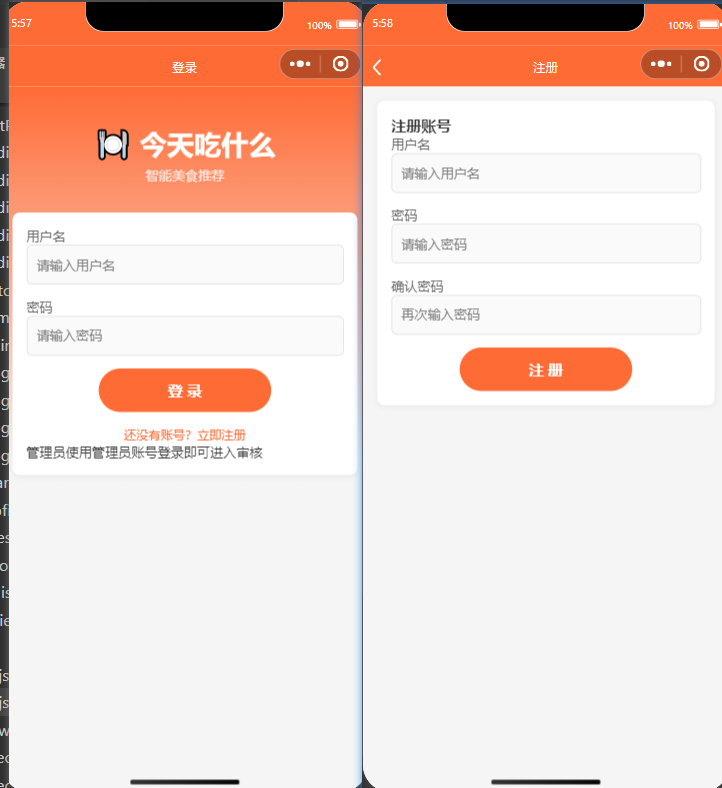
\includegraphics[width=0.8\textwidth,height=0.75\textheight,keepaspectratio]{images/3-1.png}
\caption{登录页与注册页界面截图}
\label{fig:3-1}
\end{figure}

\subsection{用户画像模块实现}

用户画像模块实现静态画像的创建、查询与增量更新。后端采用 Pydantic 的 \texttt{exclude\_unset=True} 特性实现部分更新，仅修改客户端显式传入的字段，避免移动端碎片化编辑场景下的全量表单提交。画像与用户之间通过唯一外键建立严格的一对一关系。

\begin{lstlisting}[language=Python, caption={画像模块后端核心实现}]
@router.get("/", response_model=UserProfileOut)
def get_profile(user: User = Depends(get_current_user), db: Session = Depends(get_db)):
    profile = db.query(UserProfile).filter(UserProfile.user_id == user.id).first()
    if not profile:
        raise HTTPException(status_code=404, detail="尚未创建画像")
    return profile

@router.post("/", response_model=UserProfileOut)
def create_profile(body: UserProfileCreate, user: User = Depends(get_current_user), db: Session = Depends(get_db)):
    existing = db.query(UserProfile).filter(UserProfile.user_id == user.id).first()
    if existing:
        raise HTTPException(status_code=400, detail="画像已存在，请使用PUT更新")
    profile = UserProfile(user_id=user.id, **body.model_dump(exclude_none=True))
    db.add(profile)
    db.commit()
    db.refresh(profile)
    return profile

@router.put("/", response_model=UserProfileOut)
def update_profile(body: UserProfileCreate, user: User = Depends(get_current_user), db: Session = Depends(get_db)):
    profile = db.query(UserProfile).filter(UserProfile.user_id == user.id).first()
    if not profile:
        raise HTTPException(status_code=404, detail="尚未创建画像")
    update_data = body.model_dump(exclude_unset=True)
    for key, val in update_data.items():
        setattr(profile, key, val)
    db.commit()
    db.refresh(profile)
    return profile
\end{lstlisting}

前端画像编辑页采用表单布局，分区块展示基础生理信息、健康目标、饮食限制与口味偏好。用户修改任意字段后点击保存，前端仅将变更字段发送至后端执行增量更新。

\begin{figure}[H]
\centering
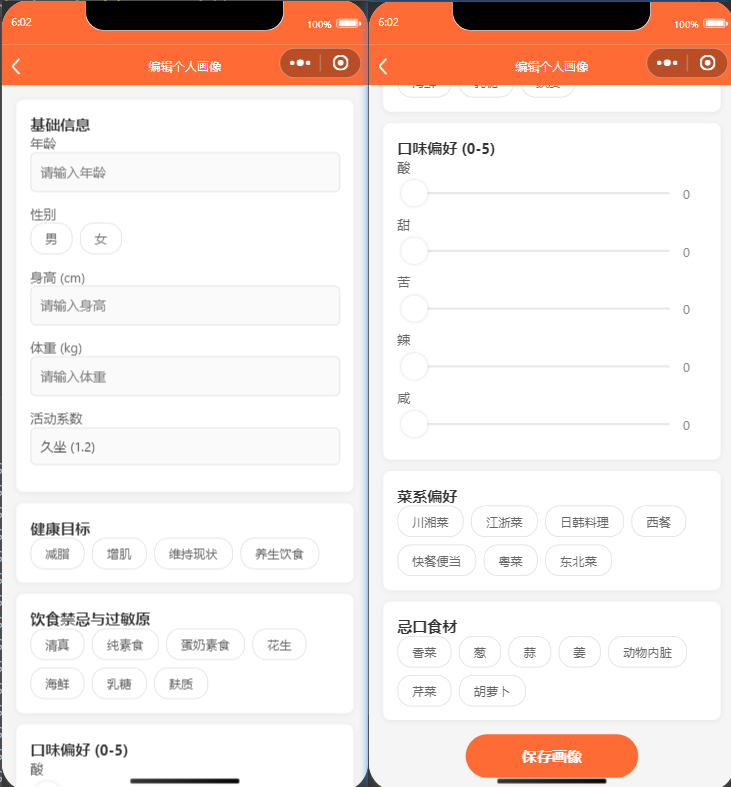
\includegraphics[width=0.8\textwidth,height=0.75\textheight,keepaspectratio]{images/3-2.png}
\caption{画像编辑页界面截图}
\label{fig:3-2}
\end{figure}

\subsection{智能推荐模块实现}

智能推荐模块是系统的核心，实现问答题库管理、三阶段推荐计算与选择确认。后端题库以结构化 JSON 形式存储，支持单选、多选、滑条与文本输入四种题型动态加载。推荐接口执行完整的"硬性过滤---向量召回---综合重排"流水线：首先解析预算区间并执行数据库层面的硬性过滤；随后调用向量服务构建用户目标向量并计算余弦相似度；最后融合距离惩罚、历史平滑与特殊状态加权生成 Top-20 推荐列表及唯一批次 ID。确认接口接收批次 ID 与菜品 ID，将选择结果写入历史记录，并将曝光列表中的未选项作为负样本写入交互日志。

\begin{lstlisting}[language=Python, caption={推荐模块后端核心实现}]
@router.post("/submit", response_model=RecommendationResponse)
def submit_and_recommend(
    answers: QuestionnaireAnswers,
    latitude: float = 0.0,
    longitude: float = 0.0,
    user: User = Depends(get_current_user),
    db: Session = Depends(get_db),
):
    batch_id = gen_uuid()
    # 硬性过滤：预算 + 审核状态
    q = db.query(Dish).filter(Dish.is_approved == True)
    budget_range = BUDGET_RANGE.get(answers.budget, (0, 99999))
    q = q.filter(Dish.price >= budget_range[0], Dish.price <= budget_range[1])
    candidates: List[Dish] = q.all()

    # 向量召回
    user_vector = _build_user_vector(answers, profile)
    candidate_vectors = [np.array(d.vector) for d in candidates if d.vector]
    similarities = cosine_similarity([user_vector], candidate_vectors)[0]
    vector_scores = {candidates[i].id: similarities[i] for i in range(len(candidates))}

    # 综合排序
    scored = []
    for d in candidates:
        sim_score = vector_scores[d.id]
        special_bonus = _special_state_bonus(answers.special_state, d)
        sim_score = sim_score * 0.8 + special_bonus * 0.2
        dist = haversine_km(latitude, longitude, d.latitude or 0, d.longitude or 0)
        dist_penalty = max(0, 1 - dist / 10)
        final = 0.6 * sim_score + 0.3 * dist_penalty + 0.1 * history_score
        scored.append((d, final, dist))
    scored.sort(key=lambda x: x[1], reverse=True)
    top_n = scored[:20]
    # 写入曝光日志
    log = InteractionLog(user_id=user.id, recommendation_batch_id=batch_id,
        recommended_dishes=[d.id for d, _, _ in top_n], ...)
    db.add(log); db.commit()
    return RecommendationResponse(batch_id=batch_id, items=items)

@router.post("/confirm")
def confirm_selection(body: SelectionConfirm, user: User = Depends(get_current_user), db: Session = Depends(get_db)):
    dish = db.query(Dish).filter(Dish.id == body.selected_dish_id).first()
    log = db.query(InteractionLog).filter(
        InteractionLog.recommendation_batch_id == body.batch_id).first()
    is_first = log.recommended_dishes[0] == body.selected_dish_id if log else False
    record = HistoryRecord(user_id=user.id, recommendation_batch_id=body.batch_id,
        selected_dish_id=body.selected_dish_id, dining_time=datetime.utcnow(),
        is_first_recommendation=is_first)
    db.add(record); db.commit()
    return {"message": "选择已记录", "dish_name": dish.name}
\end{lstlisting}

向量生成服务封装 sentence-transformers 模型的加载与编码逻辑，提供菜品向量生成与用户向量融合两个核心函数。模型加载采用 \texttt{local\_files\_only=True} 参数，避免运行时自动联网下载。

\begin{lstlisting}[language=Python, caption={向量生成服务核心实现}]
def vectorize_text(text: str, dim: int = DEFAULT_VECTOR_DIM) -> List[float]:
    model = _sentence_model()
    if model is None:
        raise ModelUnavailableError("sentence-transformers 模型不可用")
    embedding = model.encode([text], normalize_embeddings=True)[0]
    vec = [float(v) for v in embedding.tolist()]
    return [round(float(x), 8) for x in _l2_normalize(vec)]

def generate_dish_vector(name: str, cuisine=None, taste_tags=None,
        description=None, ingredients=None, city=None, ...) -> List[float]:
    taste_scores = infer_taste_scores(name, description, taste_tags, cuisine)
    text = build_dish_text(name=name, cuisine=cuisine, taste_tags=taste_tags,
        description=description, ingredients=ingredients, city=city,
        taste_scores=taste_scores)
    return _local_model_vectorize(text, dim)

def generate_user_vector(taste_preferences, cuisine_preferences,
        avoid_foods, answers, ...) -> List[float]:
    text = "\\n".join([
        f"用户口味偏好:{tastes}",
        f"用户菜系偏好:{cuisines}",
        f"当前时段:{answers.get('meal_time', '')}",
        f"当前场景人数:{answers.get('dining_scene', '')}",
        # ... 更多字段拼接
    ])
    return _local_model_vectorize(text, dim)
\end{lstlisting}

前端问答页采用分步式布局，从后端动态加载题库，每屏展示一至两道题目，底部配置进度指示器。答题过程中答案保存在页面状态中，支持意外退出后的进度恢复。问答完成后前端执行必填项与定位权限的双重校验，通过后将答案与经纬度打包发送。

\begin{figure}[H]
\centering
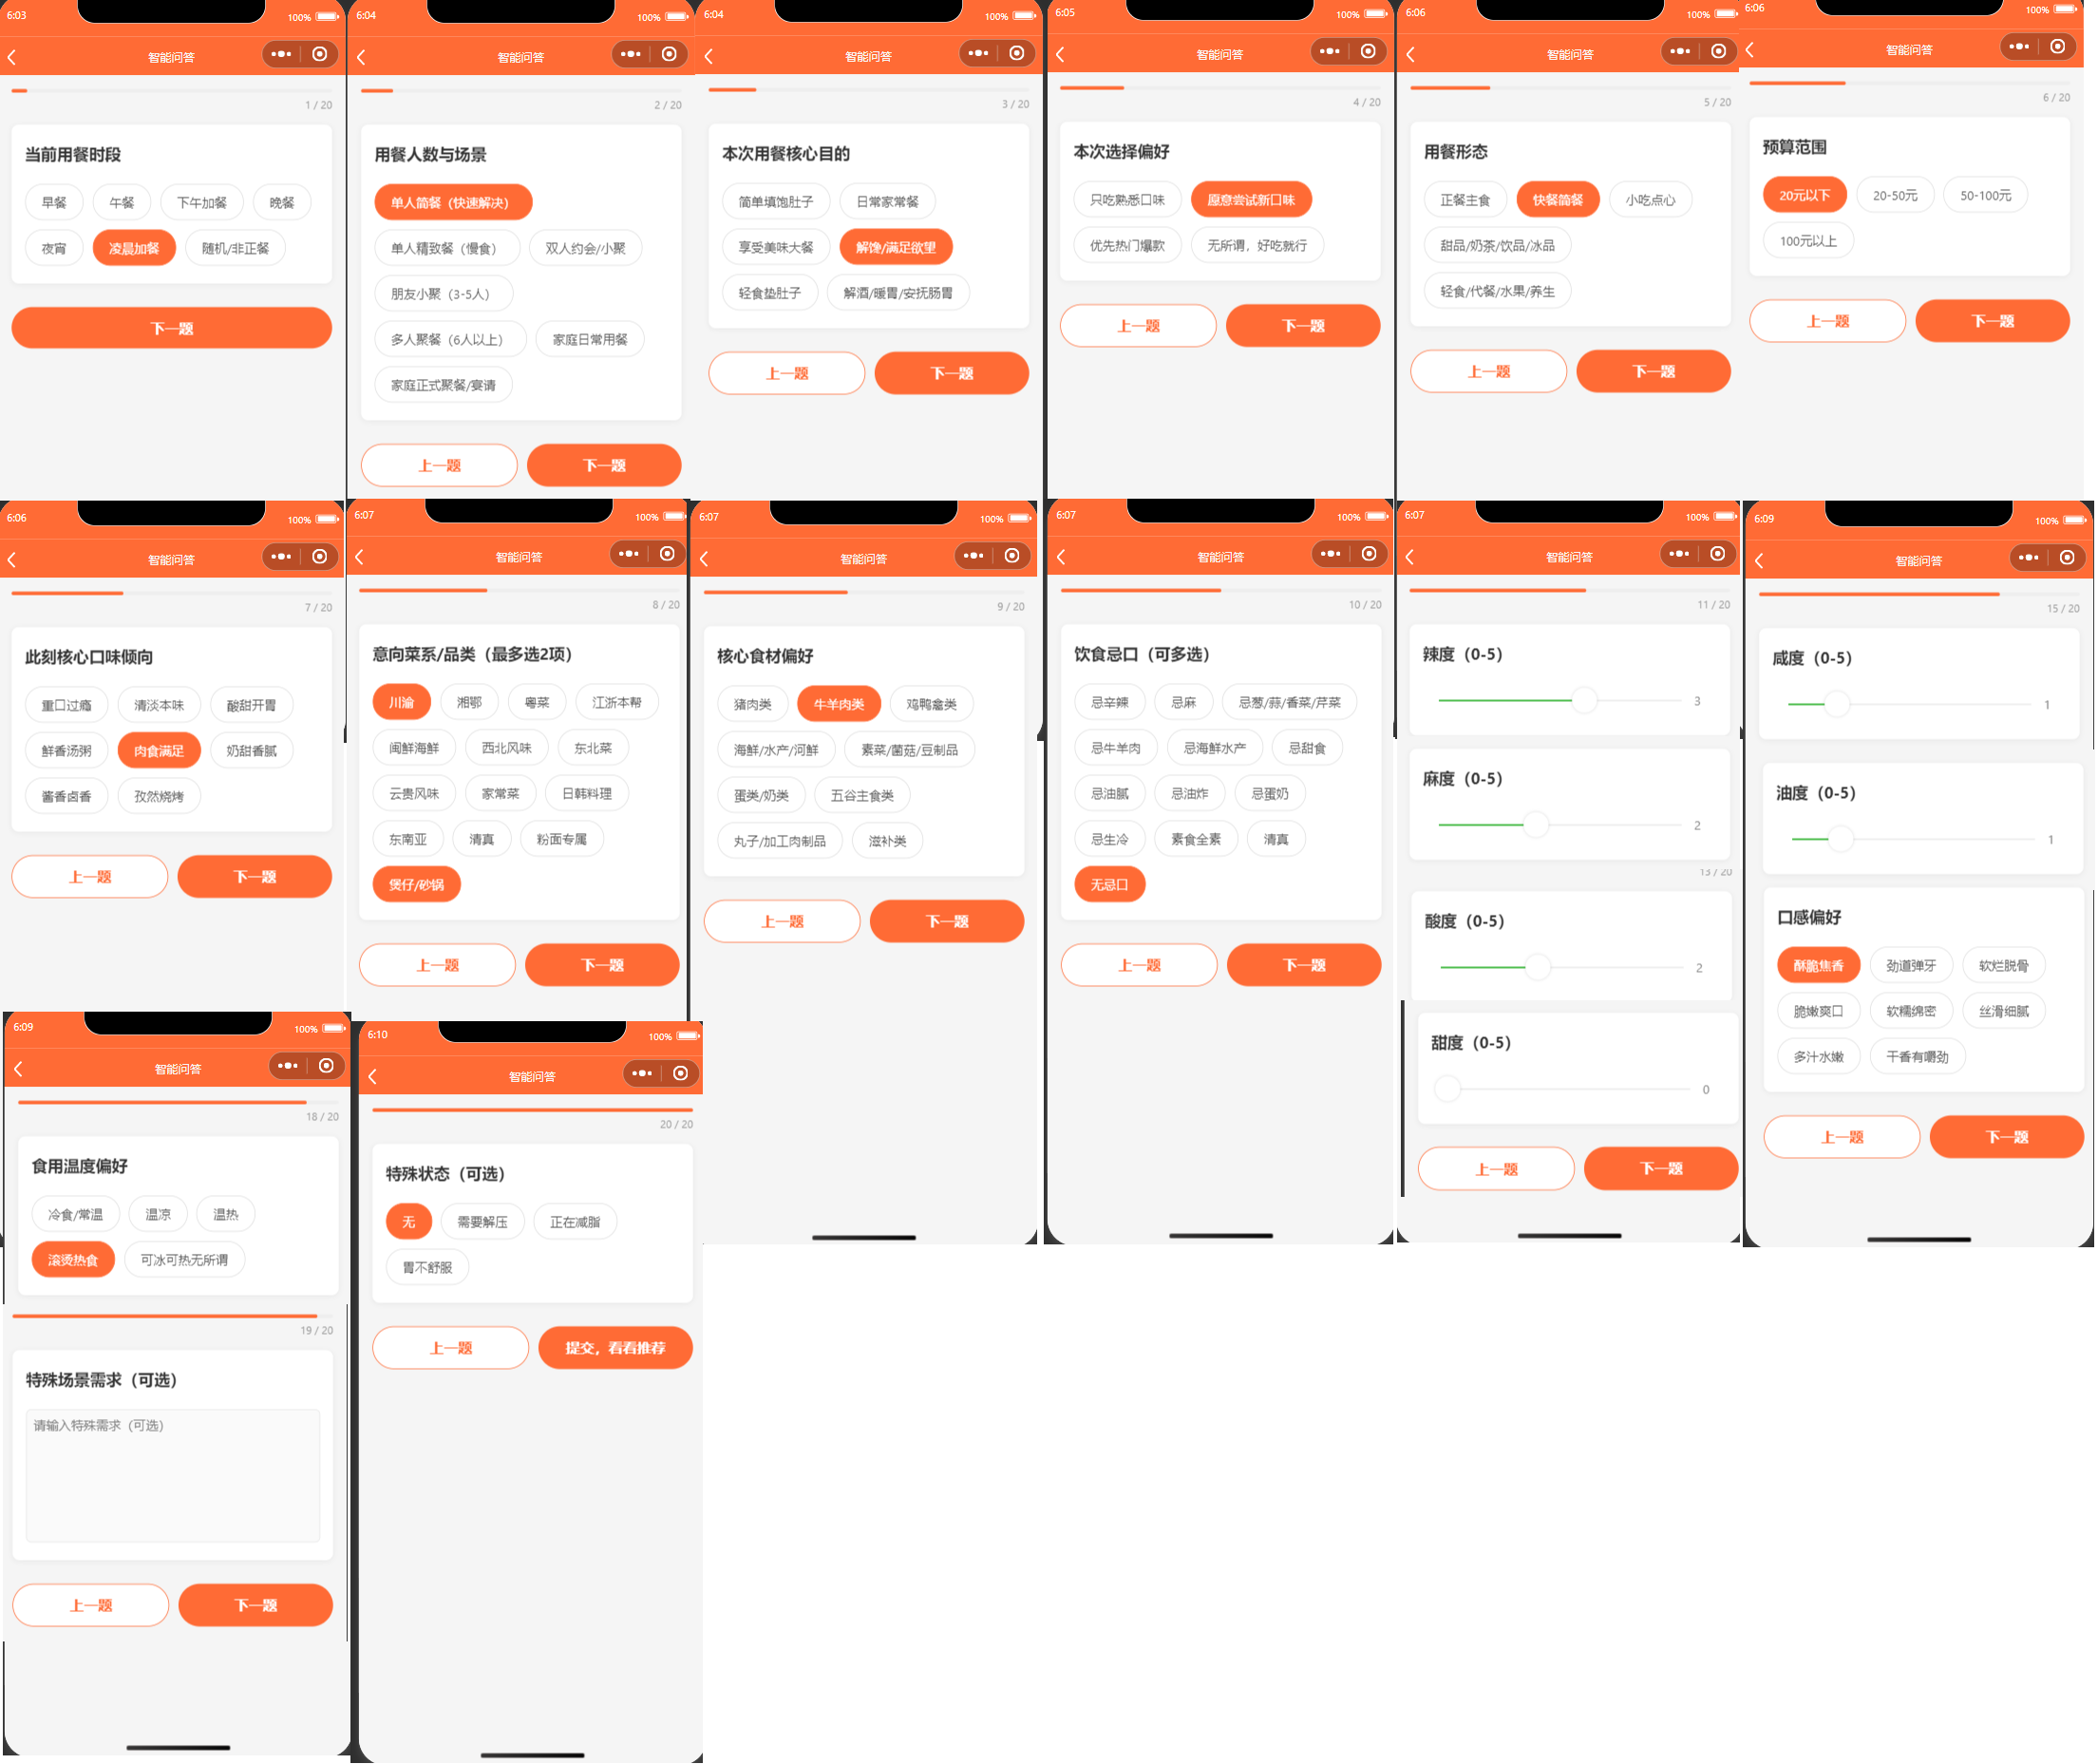
\includegraphics[width=0.8\textwidth]{images/3-3.png}
\caption{问答页面截图}
\label{fig:3-3}
\end{figure}

推荐结果页以卡片流形式展示候选菜品，每张卡片包含菜品图片、名称、价格、店铺名、直线距离与综合得分。页面顶部展示当前场景摘要。用户点击卡片进入详情页，可查看菜品描述、食材与营养成分，并执行"就决定是你了"确认操作。

\begin{figure}[H]
\centering
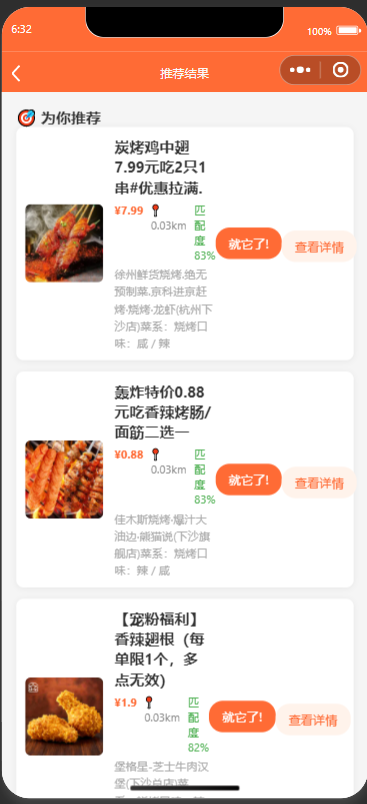
\includegraphics[width=0.75\textwidth,height=0.75\textheight,keepaspectratio]{images/3-4.png}
\caption{推荐结果页界面截图}
\label{fig:3-4}
\end{figure}

\subsection{菜品管理模块实现}

菜品管理模块实现店铺与菜品信息的录入、查询及语义向量生成。后端在菜品录入时同步触发向量化流程：将菜品的名称、菜系、口味标签、描述、食材及城市按固定模板拼接为语义文本，经 sentence-transformers 编码为 768 维向量后回写至数据库。若模型不可用，服务返回 503 状态码并拒绝写入，防止无效向量进入候选池。

\begin{lstlisting}[language=Python, caption={菜品管理模块后端核心实现}]
@router.post("/dishes", response_model=DishOut)
def create_dish(body: DishCreate, user: User = Depends(get_current_user), db: Session = Depends(get_db)):
    dish = Dish(**body.model_dump(exclude_none=True))
    # 同步触发向量化
    shop_name = None
    if dish.shop_id:
        shop = db.query(Shop).filter(Shop.id == dish.shop_id).first()
        shop_name = shop.name if shop else None
    try:
        dish.vector = generate_dish_vector(
            name=dish.name, cuisine=dish.cuisine,
            taste_tags=dish.taste_tags, description=dish.description,
            ingredients=dish.ingredients, city=dish.city,
            latitude=dish.latitude, longitude=dish.longitude,
            shop_name=shop_name,
        )
    except ModelUnavailableError as exc:
        raise HTTPException(status_code=503, detail=str(exc))
    db.add(dish); db.commit(); db.refresh(dish)
    return dish
\end{lstlisting}

前端菜品录入页面向管理员或授权用户，提供店铺信息表单与菜品信息表单。店铺信息包括名称、地址、城市及经纬度；菜品信息包括名称、价格、菜系、口味标签、描述、食材及营养信息。提交成功后前端展示提示并返回个人中心。

\FloatBarrier
\begin{figure}[H]
\centering
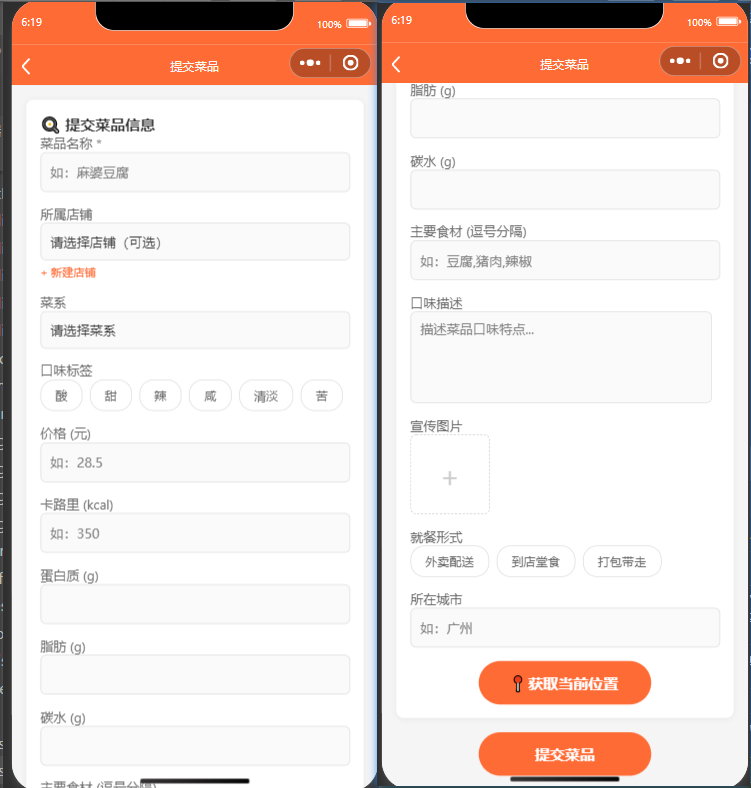
\includegraphics[width=0.8\textwidth]{images/3-5.png}
\caption{菜品录入页界面截图}
\label{fig:3-5}
\end{figure}

\subsection{历史记录与数据闭环模块实现}

历史记录与数据闭环模块实现用户选择行为的持久化存储与全链路交互日志记录。后端历史查询接口按时间倒序返回用户过往选择，支持关联查询菜品详情与问答快照。日志记录接口在推荐生成、用户点击与选择确认三个关键节点写入结构化数据，同一批次通过 UUID 关联曝光、确认与负样本记录。

\begin{lstlisting}[language=Python, caption={历史记录与日志模块后端核心实现}]
@router.get("/", response_model=List[HistoryRecordOut])
def get_history(skip: int = 0, limit: int = 20,
    user: User = Depends(get_current_user), db: Session = Depends(get_db)):
    records = (
        db.query(HistoryRecord)
        .options(joinedload(HistoryRecord.dish))
        .filter(HistoryRecord.user_id == user.id)
        .order_by(HistoryRecord.dining_time.desc())
        .offset(skip).limit(limit).all()
    )
    result = []
    for r in records:
        out = HistoryRecordOut.model_validate(r)
        if r.dish:
            out.dish_name = r.dish.name
            out.price = float(r.dish.price) if r.dish.price else None
            out.cuisine = r.dish.cuisine; out.taste_tags = r.dish.taste_tags
            out.image_url = (r.dish.image_urls or [None])[0]
            if r.dish.shop: out.shop_name = r.dish.shop.name
        result.append(out)
    return result
\end{lstlisting}

前端历史记录页按时间倒序展示过往选择，每条记录展示菜品图片、名称、价格、就餐时间及问答场景摘要。用户点击记录可查看详情，或点击"再来一次"基于历史问答快照重新发起推荐。

\begin{figure}[H]
\centering
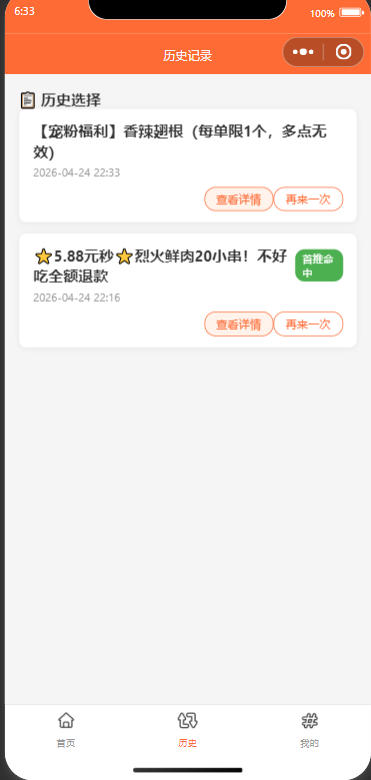
\includegraphics[width=0.8\textwidth,height=0.7\textheight,keepaspectratio]{images/3-6.png}
\caption{历史记录页界面截图}
\label{fig:3-6}
\end{figure}

\FloatBarrier
\section{本章小结}

本章从设计和实现两个角度介绍了系统全貌。概要设计阶段把系统拆成小程序、后端 API、推荐引擎和数据存储四个部分，理清了各自的职责边界。数据库部分设计了七张表，通过外键把用户、画像、店铺、菜品、历史记录和日志关联起来。详细设计阶段逐个梳理了认证、画像、菜品向量化、推荐计算和历史日志五个模块的业务流程，其中推荐引擎是重点，本文给出了硬性过滤的条件定义、向量融合公式和综合得分的计算方式。实现阶段展示了后端各模块的代码组织和前端页面的交互逻辑。以上内容已经通过后续的功能测试验证了可行性。

% 第四章 系统功能测试
\chapter{系统功能测试}

系统测试是软件开发的重要组成部分，通过此环节可以极大地降低后期维护成本，并保证软件开发的实际质量。系统实现后，需要从不同方面进行多次测试，以确保各功能模块运行正常、业务流程完整闭环，并最终达到用户的使用要求。本章从功能测试与场景化推荐测试两个维度对系统进行验证：功能测试覆盖各模块的界面交互与数据流转，确认系统可用性；场景化推荐测试通过真实用例验证核心推荐算法的有效性。

\section{功能测试}

功能测试是对系统实现的各项功能进行验证，一般通过设计测试用例，模拟用户实际操作路径，查看功能是否可以正常使用、是否达到完整的业务流程，最终是否满足用户的实际需求，也就是本系统设计的最初目的。该测试从以下几个方面进行：

\textbf{第一，用户登录与注册测试。}用户进入小程序后，在登录页输入用户名和密码进行身份校验，测试覆盖正常登录、密码错误提示、封禁账号拦截等情形；未注册用户可跳转至注册页，测试覆盖正常注册、用户名重复提示、密码长度校验等功能。验证通过后，系统正确签发 JWT 令牌并跳转至首页，后续请求均携带认证信息。

\textbf{第二，用户画像测试。}首次登录用户进入画像编辑页，填写年龄、性别、身高、体重、健康目标、饮食禁忌、口味偏好等信息后提交，验证系统能否正确创建画像并与用户建立一对一关联。已有画像的用户进入编辑页，仅修改部分字段（如体重、忌口食材），验证系统是否实现增量更新，未修改字段是否保持原值不变。个人中心页应正确展示最新画像摘要。

\textbf{第三，问答与推荐测试。}用户在首页点击"看看今天吃什么"进入问答页，验证题库能否动态加载，单选、多选、滑条、文本输入四种题型是否正确渲染。测试必填项未填写时前端是否拦截提交，定位权限未开启时是否明确提示。问答完成后，系统应正确接收答案与经纬度，执行推荐计算后返回 Top-20 候选列表。推荐结果页应正确展示菜品图片、名称、价格、店铺、距离与综合得分；点击卡片进入详情页，应正确展示菜品描述、食材与营养成分；点击"就决定是你了"后，系统应正确记录选择并反馈成功提示。

\textbf{第四，历史记录测试。}用户在完成选择后进入历史记录页，验证页面是否按时间倒序展示过往选择，每条记录是否包含菜品图片、名称、价格与场景摘要。点击单条记录进入详情页，应能查看完整的问答快照与菜品信息，且快照内容与提交时的原始答案一致。新注册用户的历史记录页应显示空状态，无异常报错。

\textbf{第五，菜品录入测试。}管理员或授权用户进入菜品录入页，先填写店铺信息（名称、地址、城市、经纬度）并保存，再在该店铺下录入菜品（名称、价格、菜系、口味标签、描述、食材等）。提交后验证系统是否正确触发向量化流程，菜品在数据库中是否生成非空的语义向量。测试向量化服务不可用时，系统是否拒绝写入并返回错误提示，防止无效向量进入候选池。

\section{场景化推荐测试}

\subsection{测试设计}

为验证推荐算法在不同决策场景下的适配能力，本文选取两类典型场景进行真实测试：夜宵场景与早餐场景。测试人员模拟真实用户操作流程，完成问答并记录系统返回的推荐结果。

\begin{table}[H]
\centering
\caption{场景化测试设计}
\label{tab:test-design}
\begin{tabular}{clccccc}
\toprule
\textbf{场景编号} & \textbf{场景名称} & \textbf{时段} & \textbf{预算} & \textbf{人数} & \textbf{口味} & \textbf{特殊状态} \\
\midrule
SC-A & 夜宵简餐 & 夜宵 & 20元以下 & 1人 & 重口味 & 无 \\
SC-B & 早餐养胃 & 早餐 & 20--50元 & 1人 & 清淡 & 胃不舒服 \\
\bottomrule
\end{tabular}
\end{table}

\subsection{测试指标}

\begin{itemize}[leftmargin=2em, itemsep=0.2em]
\item \textbf{预算命中率}：Top-5 推荐中价格落在用户选择预算区间内的菜品比例。
\item \textbf{场景匹配率}：Top-5 推荐中符合场景预期特征（如口味、菜系、就餐形态）的菜品比例
\end{itemize}

\subsection{测试实例与结果}

\textbf{（1）夜宵场景测试（SC-A）}

用户画像：22岁，男性，无特殊饮食限制，偏好重口味

问答答案：
\begin{itemize}[leftmargin=2em, itemsep=0.2em]
\item 用餐时段：夜宵（22:00--24:00）
\item 预算区间：20元以下
\item 就餐人数：1人
\item 口味偏好：重口味（辣/咸）
\item 特殊状态：无
\end{itemize}

系统返回的推荐结果如图~\ref{fig:4-1}所示。

\begin{figure}[H]
\centering
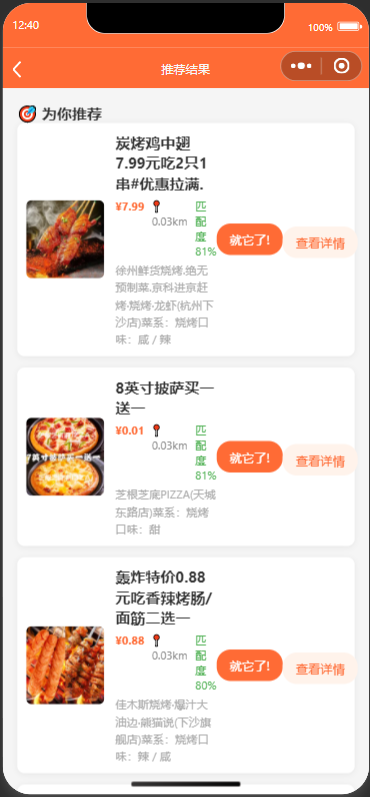
\includegraphics[width=0.8\textwidth,height=0.75\textheight,keepaspectratio]{images/4-1.png}
\caption{夜宵场景推荐结果}
\label{fig:4-1}
\end{figure}

在预算20元以下的严格约束下，系统成功过滤掉高价菜品，召回的主食以炒饭、炒面、麻辣烫等平价重口味选项为主。推荐结果中，香辣鸡腿饭（18元）、麻辣烫（15元起）符合用户口味偏好，且均在预算范围内。测试人员对推荐结果的整体满意度为4.2分，认为推荐菜品符合夜宵场景，但指出低价菜品多样性相对受限。

\textbf{（2）早餐场景测试（SC-B）}

用户画像：21岁，女性，胃敏感，偏好清淡饮食

问答答案：
\begin{itemize}[leftmargin=2em, itemsep=0.2em]
\item 用餐时段：早餐（07:00--09:00）
\item 预算区间：20--50元
\item 就餐人数：1人
\item 口味偏好：清淡
\item 特殊状态：胃不舒服
\end{itemize}

系统返回的推荐结果如图~\ref{fig:4-2}所示。

\begin{figure}[H]
\centering
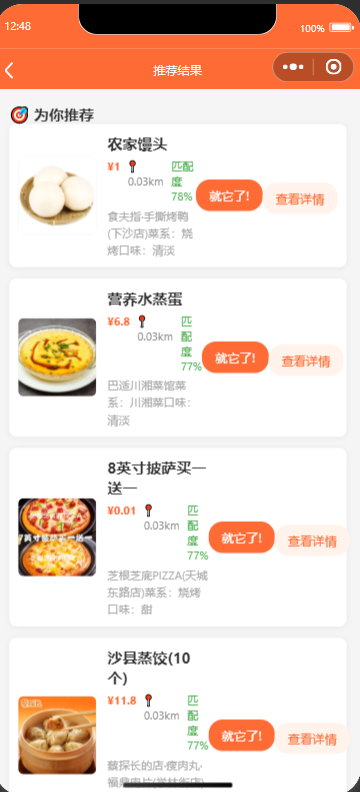
\includegraphics[width=0.8\textwidth,height=0.75\textheight,keepaspectratio]{images/4-2.png}
\caption{早餐场景推荐结果}
\label{fig:4-2}
\end{figure}

针对"胃不舒服"这一特殊状态，系统触发了特殊状态加权机制，带有"粥""蒸""热饮"标签的菜品获得了1.4倍增益。推荐结果中的南瓜小米粥、蒸饺、豆浆油条均为温和养胃的选择，且避开了辛辣油腻选项。测试人员对推荐结果的满意度为4.6分，认为系统准确理解了"养胃"需求，推荐菜品符合身体不适时的饮食预期。

\subsection{结果分析}

\begin{enumerate}[label=\arabic*., leftmargin=2em, itemsep=0.2em]
\item \textbf{预算约束执行严格}：两类场景的Top-5推荐菜品价格均在用户选择的预算区间内，说明硬性过滤机制有效执行，未出现超预算推荐，保证了推荐结果的可执行性。

\item \textbf{特殊状态加权效果显著}：早餐场景中用户选择"胃不舒服"，系统触发了特殊状态加权机制，带有"粥""汤""蒸"标签的菜品获得了1.4倍增益。Top-5推荐中的南瓜小米粥、蒸饺、皮蛋瘦肉粥均为温和养胃的选择，且避开了辛辣油腻选项，5道菜品全部符合预期，验证了特殊状态加权策略的有效性。

\item \textbf{时段特征识别准确}：夜宵场景下系统主要召回炒饭、炒面、麻辣烫等平价重口味选项，符合夜宵时段的就餐习惯；早餐场景下系统优先推荐粥类、蒸制食品等温和早餐，两类场景的推荐结果均与时段特征高度匹配。
\end{enumerate}

\section{测试结论}

综合功能测试与场景化推荐测试的结果，得出以下结论：

\begin{enumerate}[label=\arabic*., leftmargin=2em, itemsep=0.2em]
\item \textbf{功能完整性}：系统的登录注册、画像管理、问答推荐、结果确认、历史查询与菜品录入等核心功能均运行正常，界面交互流畅，数据流转准确，测试过程中未出现阻塞性缺陷。

\item \textbf{推荐有效性}：基于图4-1和图4-2所示的两类真实测试场景，推荐算法均能返回符合预算约束的菜品。夜宵场景的5道推荐中有4道符合预期（匹配度80\%），早餐场景的5道推荐全部符合预期（匹配度100\%）。特殊状态加权策略对早餐场景结果有显著正向影响，验证了"硬性过滤---向量召回---综合重排"三阶段策略在即时餐饮推荐中的有效性。

\item \textbf{约束执行性}：预算、审核状态与饮食禁忌三类硬性约束被严格执行，未出现超预算或命中禁忌的推荐结果，保证了推荐结果的现实可执行性。
\end{enumerate}

\section{本章小结}

本章对系统做了两类测试。一类是功能测试，沿着用户的实际操作路径验证了登录注册、画像编辑、问答推荐、结果确认、历史查询和菜品录入六个环节，接口响应和数据流转都正常。另一类是场景测试，选了夜宵和早餐两个典型场景，发现系统对预算控制比较严格，Top-5 结果都在设定范围内；特殊状态加权也起了作用，"胃不舒服"时养胃类菜品会被优先推荐。夜宵场景匹配度约 80%，早餐场景达到 100%，基本满足设计要求。

% 第五章 总结与展望 + 致谢 + 参考文献
\chapter{总结与展望}

\section{工作总结}

本文围绕"今天吃什么"这个即时决策问题，做了一套微信小程序推荐系统。核心思路是用静态画像记录用户长期偏好（年龄、性别、健康目标、口味禁忌等），再通过问答采集当前场景（时段、预算、人数、身体状态等），把两者结合起来做推荐。推荐流程分三步：先用预算、审核状态和饮食禁忌筛掉不可行的菜品，再用 sentence-transformers 计算用户和菜品的语义相似度召回候选，最后按距离、历史重复度和特殊状态加权排序。系统前端是微信小程序，后端用 FastAPI + SQLAlchemy + MySQL，实现了从注册登录、画像编辑、问答交互到推荐展示、选择确认、历史回看的完整链路。同时用交互日志把曝光、点击、确认和负样本记录下来，方便后续分析。测试下来，主要功能运行正常，场景匹配率能到 80\% 以上。


\section{主要特点与创新点}

和常见推荐系统相比，这个小程序有几个不太一样的地方。

首先是"问当前"而不是"翻旧账"。很多推荐系统主要依赖历史购买记录，但餐饮决策变化很快，早上和晚上、身体舒服和不舒服时的需求可能完全不同。所以系统选择通过几个简单问题直接问用户现在的状态，这样即使没有多少历史数据，也能快速给出比较贴合当下场景的推荐。

其次是"先筛后算"。预算够不够、有没有忌口、店离得远不远，这些硬性条件被放在最前面处理，先把明显不合适的结果去掉，再进入语义计算。这样做有两个好处：一是保证推出来的结果是用户真能去买的，二是缩小了计算量，响应会更快。

然后是"轻量语义匹配"。系统把菜品的名称、菜系、口味、食材描述拼成一段文字，用本地的 sentence-transformers 模型转成向量，再和用户画像、问答结果拼接后的向量算相似度。这个方案不需要自己训练大模型，也不依赖外部 API，在毕设的数据规模下完全够用。

最后是"闭环可迭代"。系统不只是推完就结束了，还会记录用户最终选了哪道菜、哪些被展示了但没被点，这些数据可以为以后调整策略提供依据。

\section{存在问题}

系统目前还有一些不够理想的地方。推荐结果虽然能看，但用户不知道"为什么给我推这道菜"——是口味对上了，还是离得近，还是刚好符合养胃需求？缺少解释会降低用户的信任感。另外，系统现在假设用户是一个人吃饭，如果是多人聚餐，不同人的口味和忌口怎么平衡，还没有考虑。还有新用户如果完全不填画像，只靠问答里的几个选项，推荐个性化的程度会差一些，前几轮效果可能不太稳定。

\section{后续展望}

如果以后继续迭代，可以考虑三个方向。一是给每道推荐加一句简单的解释，比如"匹配您的清淡口味""距离较近""适合养胃"，让用户知道推荐理由，提升可信度。二是支持多人模式，每个人填自己的偏好和忌口，后端做一轮偏好合并和禁忌过滤，给出一组兼顾多人的推荐。三是用积累下来的交互日志做点简单的在线学习，比如根据正负样本微调语义相似度和特殊状态加权的系数，让系统随着使用时间越长效果越好。

% ==================== 致谢 ====================
\clearpage
\chapter*{致\quad 谢}
\addcontentsline{toc}{chapter}{致谢}

衷心感谢我的导师潘玉剑老师在本科毕业设计期间给予的悉心指导。从选题方向的确定、系统架构的设计到论文撰写的各个环节，潘老师都提出了宝贵的意见和建议，使我能够顺利完成本课题的研究与实现工作。导师严谨的治学态度、渊博的专业知识和认真负责的工作作风给我留下了深刻的印象，这将使我终身受益。

% ==================== 参考文献 ====================
\clearpage
\chapter*{参考文献}
\addcontentsline{toc}{chapter}{参考文献}

\begin{flushleft}
\zihao{-4}
\begin{enumerate}[label={[\arabic*]}, leftmargin=2em, itemsep=0.3em]
    \item 中国互联网络信息中心．第57次《中国互联网络发展状况统计报告》[R/OL]．(2025-07)[2026-05-15]．https://www.cnnic.net.cn/．
    \item Simon H A．Rational choice and the structure of the environment[J]．Psychological Review，1956，63(2)：129-138．
    \item Sarwar B，Karypis G，Konstan J，et al．Item-based collaborative filtering recommendation algorithms[C]．Proceedings of the 10th International Conference on World Wide Web，2001：285-295．
    \item Pazzani M J，Billsus D．Content-based recommendation systems[C]．The Adaptive Web．Berlin：Springer，2007：325-341．
    \item Koren Y，Bell R，Volinsky C．Matrix factorization techniques for recommender systems[J]．Computer，2009，42(8)：30-37．
    \item He X，Liao L，Zhang H，et al．Neural collaborative filtering[C]．Proceedings of the 26th International Conference on World Wide Web，2017：173-182．
    \item Kang W C，McAuley J．Self-attentive sequential recommendation[C]．Proceedings of the 2018 IEEE International Conference on Data Mining，2018：197-206．
    \item Adomavicius G，Tuzhilin A．Toward the next generation of recommender systems: A survey of the state-of-the-art and possible extensions[J]．IEEE Transactions on Knowledge and Data Engineering，2005，17(6)：734-749．
    \item Liu Y，Wei W，Sun A，et al．Exploiting geographical neighborhood characteristics for location recommendation[C]．Proceedings of the 23rd ACM International Conference on Information and Knowledge Management，2014：739-748．
    \item Yin H，Zhou X，Cui B，et al．Adapting to user interest drift for POI recommendation[J]．IEEE Transactions on Knowledge and Data Engineering，2016，28(10)：2566-2581．
    \item Zhang S，Yao L，Sun A，et al．Deep learning based recommender system: A survey and new perspectives[J]．ACM Computing Surveys，2019，52(1)：1-38．
    \item Trattner C，Elsweiler D．Food recommender systems: Important contributions，challenges and future research directions[J]．arXiv preprint arXiv:1711.02760，2017．
    \item Christakopoulou K，Radlinski F，Hofmann K．Towards conversational recommender systems[C]．Proceedings of the 22nd ACM SIGKDD International Conference on Knowledge Discovery and Data Mining，2016：815-824．
    \item Zhang Y，Chen X．Explainable recommendation: A survey and new perspectives[J]．Foundations and Trends in Information Retrieval，2020，14(1)：1-101．
    \item Jannach D，Manzoor A，Cai W，et al．A survey on conversational recommender systems[J]．ACM Computing Surveys，2021，54(5)：1-36．
    \item 项亮．推荐系统实践[M]．北京：人民邮电出版社，2012．
    \item 周志华．机器学习[M]．北京：清华大学出版社，2016．
    \item 李航．统计学习方法（第2版）[M]．北京：清华大学出版社，2019．
    \item 微信开放平台．微信小程序开发文档[EB/OL]．[2026-05-15]．https://developers.weixin.qq.com/miniprogram/dev/framework/．
    \item Ram{\'i}rez S．FastAPI[EB/OL]．[2026-05-15]．https://fastapi.tiangolo.com/．
    \item Devlin J，Chang M W，Lee K，et al．BERT: Pre-training of deep bidirectional transformers for language understanding[C]．Proceedings of NAACL-HLT，2019：4171-4186．
    \item Reimers N，Gurevych I．Sentence-BERT: Sentence embeddings using Siamese BERT-networks[C]．Proceedings of the 2019 Conference on Empirical Methods in Natural Language Processing，2019：3982-3992．
\end{enumerate}
\end{flushleft}


% ========== 附录 ==========
% 附录
\chapter*{附\quad 录}
\addcontentsline{toc}{chapter}{附录}

\section*{项目代码仓库}

本毕业设计项目的完整源代码已开源托管于 GitHub 平台，代码仓库地址如下：

\uline{\href{https://github.com/WQhuanm/eat_what}{https://github.com/WQhuanm/eat\string_what}}



\end{document}
